% \documentclass[review]{elsarticle}
\documentclass[utf8, babel, sor, jor, amsmath, amssymb, reprint]{elsarticle} %удалить перед отправкой
\usepackage{comment} %удалить перед отправкой
\usepackage[T2A]{fontenc} %удалить перед отправкой
\usepackage[utf8x]{inputenc} %удалить перед отправкой
\usepackage[english,russian]{babel} %удалить перед отправкой
\graphicspath{{images/}}

\usepackage{lineno,hyperref}
\usepackage{algorithm}
\usepackage{algorithmic}
\modulolinenumbers[5]

\journal{Journal of \LaTeX\ Templates}

\bibliographystyle{elsarticle-num}

\usepackage{mathrsfs}
\usepackage{amsmath}
\usepackage{amssymb}%
\usepackage{multirow}



%%%%%%%%%%%%%%%%%%%%%%%
%% Elsevier bibliography styles
%%%%%%%%%%%%%%%%%%%%%%%
%% To change the style, put a % in front of the second line of the current style and
%% remove the % from the second line of the style you would like to use.
%%%%%%%%%%%%%%%%%%%%%%%

%% Numbered
%\bibliographystyle{model1-num-names}

%% Numbered without titles
%\bibliographystyle{model1a-num-names}

%% Harvard
%\bibliographystyle{model2-names.bst}\biboptions{authoryear}

%% Vancouver numbered
%\usepackage{numcompress}\bibliographystyle{model3-num-names}

%% Vancouver name/year
%\usepackage{numcompress}\bibliographystyle{model4-names}\biboptions{authoryear}

%% APA style
%\bibliographystyle{model5-names}\biboptions{authoryear}

%% AMA style
%\usepackage{numcompress}\bibliographystyle{model6-num-names}

%% `Elsevier LaTeX' style
\bibliographystyle{elsarticle-num}
%%%%%%%%%%%%%%%%%%%%%%%


\usepackage{xcolor}
\newcommand{\todo}[1] {\textcolor{red}{#1}} %%for TODO comments
\def\l{\left\langle}
\def\r{\right\rangle}
\usepackage{mathrsfs}
\usepackage{amsmath}
\usepackage{amssymb}%

\begin{document}

\begin{frontmatter}


\title{Frustrations in the ground state of the $\pm J$ Ising model on a square lattice}

\author[mainaddress, secondaryaddress]{Viacheslav Trukhin\corref{mycorrespondingauthor}}
\ead{trukhin.vo@dvfu.ru}

\author[mainaddress]{Egor Prokhorov\corref{mycorrespondingauthor}}
\ead{prokhorov.ei@dvfu.ru}

\author[mainaddress, secondaryaddress]{Aleksandr Makarov\corref{mycorrespondingauthor}}
\ead{makarov.ag@dvfu.ru}

\author[mainaddress, secondaryaddress]{Konstantin Nefedev\corref{mycorrespondingauthor}}
\ead{nefedev.kv@dvfu.ru}


\address[mainaddress]{Far Eastern Federal University, Vladivostok, Russky Island, 10 Ajax Bay, 690922, the Russian Federation}
\address[secondaryaddress]{Institute of Applied Mathematics, Far Eastern Branch, Russian Academy of Science, Vladivostok, Radio 7, 690041, the Russian Federation}

\begin{abstract}

By the method of exhaustive enumeration, all possible states of the Edwards-Anderson model on a simple square lattice of 8×8 spins were accurately calculated. The ground-state energy for the studied finite-size samples was determined. The macroscopic degeneracy of the ground state in frustrated spin systems is due to the combinatorics of frustrated plaquettes, i.e., the number of ways to place frustrated spin pairs on the lattice. The algorithm for calculating energy, spin excess, and ground-state configurations is based on identifying the arrangement of frustrations. The dependence of the ground-state spin excess in the Edwards-Anderson model on an external magnetic field has a discrete (step-like, stair-like) character. Critical values of the external magnetic field at which giant jumps in residual entropy are observed were calculated. The nature of these large entropy jumps is explained by the fact that at certain critical values of the external magnetic field, the sum of several spin configurations with different interaction energies and Zeeman energies, i.e., with different values of spin excess, will have the same total energy. The degeneracy multiplicities of states with the same total energy are summed up.

\end{abstract}


\begin{highlights}  
	\item The presence of frustrations in the ground state does not necessarily lead to macroscopic degeneracy.  
	\item The effect of finite-size scaling on the entropy and energy of the ground state has been accurately computed, and the asymptotic behavior of the residual entropy has been determined.  
	\item The phenomenon of macroscopic degeneracy of the ground state is due to the arrangement of frustrated plaquettes in the lattice.  
	\item The spin excess in the ground state is determined by the lattice phase.  
\end{highlights}  


\begin{keyword}
	Ising model, Ground state, GPU and CPU high performance calculations, statistical thermodynamics.
\end{keyword}


\end{frontmatter}

\linenumbers

\newpage
\tableofcontents

\newpage
\section{Introduction}

Without exaggeration, solving models of frustrated systems, such as spin glasses and spin ice, is one of the most important research areas in statistical mechanics. The Edwards-Anderson (EA) Ising spin glass model is one of the simplest spin glass models with short-range interactions \cite{edwards1975theory}. Despite its apparent simplicity, the low-temperature properties of this model, even in 2D and especially in higher dimensions, remain poorly understood \cite{pal1996ground, hartmann2011ground, newman2022ground}. Spin lattice models with competing ferromagnetic and antiferromagnetic interactions have been studied for many years \cite{binder1986spin, mezard1987spin, lebrecht2004plaquette, valdes2012j, lebrecht2015j, fan2023searching}.

Despite many years of intensive research, the nature of the low-temperature phase of the Ising model for frustrated spin systems with a limited interaction range remains unresolved \cite{roma2010ground, newman2023proof}. Two of the most important open questions concern the properties of the ground state of spin glasses (i.e., at zero temperature), particularly the degeneracy of the ground state and the nature of low-energy excitations \cite{newman2022ground}.

The calculation of the energy, entropy, and spin excess of the ground state of a spin glass with a given Hamiltonian, even without an external magnetic field, is a highly complex optimization problem. In three dimensions, this problem is $NP$-hard \cite{barahona1982computational, hartmann2002optimization}, meaning that no known algorithm can solve the problem of spin excess, energy, and ground-state degeneracy in time proportional to a polynomial function of the linear system size, and it is widely believed that such an algorithm cannot be developed. Currently, no algorithm combines high accuracy with efficiency \cite{fan2023searching}.

The properties of spin glasses at zero temperature are typically studied using approximate methods \cite{roma2009ground, perez2012ground}. Over time, various approximate approaches for solving spin system models have been developed, but the problem remains relevant due to the lack of an exact solution \cite{rybin2022hybrid, makarova2023canonical, farias2024differentiable}. However, for some lattices, such as the triangular lattice, it is possible to obtain information about entropic and magnetic properties \cite{jurvcivsinova2024classical}.

Energy can be computed using optimization methods \cite{hartmann2002optimization, hartmann2004new}, genetic algorithms \cite{holland1992adaptation}, annealing algorithms \cite{kirkpatrick1983optimization}, multicanonical sampling methods \cite{berg1994ground, shevchenko2017multicanonical}, multi-spin cluster methods \cite{makarova2023canonical}, or parallel tempering \cite{PhysRevB.50.16444, roma2009ground}.

Entropy, or the degeneracy of the ground state, is crucial information not only for understanding the low-temperature behavior of spin glasses (or spin ice) but also for the nature of excitations. Even for the 2D Edwards-Anderson model, computing the ground state is a non-trivial problem. Approximating entropy or the degeneracy multiplicity is an even more challenging task. Methods such as the transfer matrix method \cite{PhysRevB.22.288, cheung1983equilibrium, kolan1982ground}, ballistic search \cite{hartmann2000ground}, thermodynamic integration \cite{kirkpatrick1977frustration, binder1985monte, roma2004ground}, and multicanonical sampling \cite{berg1994ground, shevchenko2017multicanonical} have been developed to address this issue. However, for finite systems with a countable number of spins, approximate methods are unlikely to be applicable.  

Spin system models on lattices provide an ideal platform for exploring complex magnetic ground states with excitations, and their investigation is important for the advancement of physics \cite{lacroix2011introduction}. This research includes determining the critical switching fields between ground states in an external magnetic field, entropy jumps during transitions between ground states, and correlation functions \cite{ramirez2004effect, rosas2004random, andriushchenko2019large}.  

Studying the energy landscape of low-energy states in spin glasses \cite{biswas2023energy} remains a pressing problem, as does research on spin ice. An intriguing question is identifying the relative fraction (or concentration) of ferromagnetic (or antiferromagnetic) exchange interactions at $T=0$ that results in a transition between ferromagnetic and spin glass states (or between antiferromagnetic and spin glass states) \cite{gruzberg2001random, honecker2001universality, picco2006strong, tsomokos2011interplay, zimmer2022role}. The thermodynamic properties and phase diagram of the ground state for molecular clusters with a small number of spins were calculated in \cite{dias2023ground}.

Ground-state configurations, as well as excitations in the ground and low-energy states of spin glasses, along with macroscopic ground-state degeneracy and residual entropy at low temperatures, are actively studied in models with long-range dipolar interactions \cite{makarova2021low, singh2024micromagnetic}. The search for spin glass ground states is not only essential for understanding the nature of disordered magnets and many other physical systems but also proves useful for solving a wide range of complex combinatorial optimization problems in various disciplines. Despite decades of effort, no algorithm with both high accuracy and efficiency has yet been developed \cite{fan2023searching}.  

Estimating the ground-state energy and understanding the nature of its macroscopic degeneracy have remained open problems for many years. At low temperatures, the spin glass in its ground state is realized solely through configurations with minimal interaction energy, while the ensemble of other configurations in the Gibbs distribution plays no role. Ground-state energies calculated by various methods in studies \cite{thouless1977solution, sherrington1975solvable, tanaka1980analytic, klein1976comparison, kirkpatrick1978infinite, karandashev2019global, palmer1999ground, campbell2004energy, roma2009ground} show significant variability.  

It will be shown below that this variability may be related to the distribution of frozen disorder in the bonds, i.e., competing ferromagnetic and antiferromagnetic interactions. For a finite number of spins, the ground-state energy strongly depends on the specific realization of the distribution $\left\lbrace J_{ij} \right\rbrace$ on the spin lattice.  

In this work, we utilized an exhaustive enumeration algorithm \cite{dias2023ground, padalko2021parallel} to solve the problem of ground-state energy for a finite number of spins, to compute the degeneracy of this state, and to determine the distribution of spin excess. The availability of an exact solution, even for a relatively small number of spins, allows for testing approximate methods. By performing exhaustive enumeration, we identified all possible states, enabling us to calculate properties in the presence of an external magnetic field.

\section{Комбинаторика плакетов}

Пусть под плакетом понимается замкнутая цепочка спинов минимальной длины \cite{lebrecht2015j}. В рассмотренных далее примерах на квадратной решётке плакетами являются элементарные квадраты, см. рисунки \ref{fig:Type1}, \ref{fig:Type2}, \ref{fig:Type3}. В модели спинового стекла Эдвардса-Андерсона плакеты можно разделить на три возможных типа. 

Если $P_+$ есть относительное количество ферромагнитных ($J_{ij}=+1$) обменных интегралов, тогда к первому типу, см. рис. \ref{fig:Type1}, относятся плакеты, в которых $P_+=0.5$. Для второго типа $P_+=0.75$ или $P_+=0.25$ (рис. \ref{fig:Type2}). Для третьего типа $P_+=1.0$ или $P_+=0.0$ (рис. \ref{fig:Type3}). Прямым и зубчатым линиям на рисунках соответствуют ферромагнитные и антиферромагнитные связи, соответственно. Белые и чёрные кружки на рисунках соответствуют спинам вверх и вниз в одной из конфигураций основного состояния.


\begin{figure}[H]
	\centering
	\begin{minipage}{0.3\textwidth}
		\centering
		\resizebox{45px}{45px}{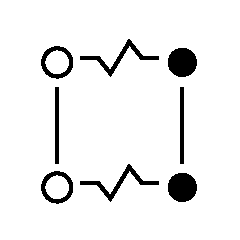
\includegraphics{pictures/Type1_1.eps}}
		\hspace{-4pt} 
		\resizebox{45px}{45px}{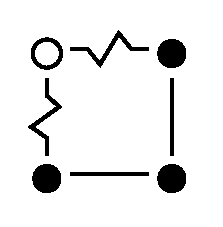
\includegraphics{pictures/Type1_2.eps}}
		\caption{Плакеты первого типа}
		\label{fig:Type1} 
	\end{minipage}
	\hspace{5pt} 
	\begin{minipage}{0.3\textwidth}
		\centering
		\resizebox{45px}{45px}{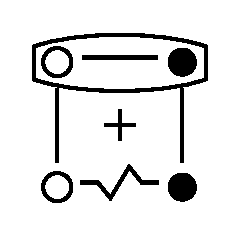
\includegraphics{pictures/Type2_1.eps}}
		\hspace{-2pt} 
		\resizebox{45px}{45px}{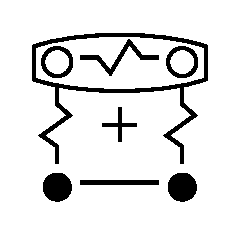
\includegraphics{pictures/Type2_2.eps}}
		\caption{Плакеты второго типа}
		\label{fig:Type2}
	\end{minipage}
	\hspace{5pt}
	\begin{minipage}{0.3\textwidth}
		\centering
		\resizebox{45px}{45px}{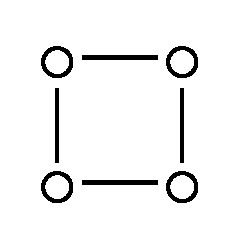
\includegraphics{pictures/Type3_1.eps}}
		\hspace{-4pt} 
		\resizebox{45px}{45px}{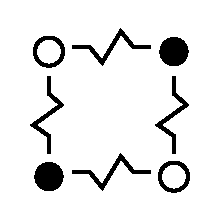
\includegraphics{pictures/Type3_2.eps}}
		\caption{Плакеты третьего типа}
		\label{fig:Type3}
	\end{minipage}
\end{figure}


В каждом из рассмотренных выше плакетов существует $2^4$ конфигураций.
Установлено, что фрустрация (возбуждение или положительная энергия обменного взаимодействия между $ij$-парой спинов) в основном состоянии обязательно появляется в плакетах второго типа, которые помечены знаком $"+"$. Причём фрустрированной парой может быть любая пара спинов.


Если система состоит из двух плакетов второго типа, например, как показано на рисунке \ref{fig:Type2_32}, то для минимизации энергии фрустрированная пара обязательно располагается на пересечении плакетов, вне зависимости от распределения обменных взаимодействий в остальной решетке. 

\begin{figure}[H]
	%\centering
	%\begin{minipage}{0.4\textwidth}
	\centering
	\begin{minipage}{0.2\textwidth}
		\centering
		(a)
		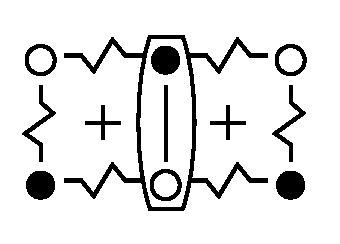
\includegraphics[width=1\textwidth]{pictures/Type2_3x2.eps}
		\label{fig:Type2_3x2}
	\end{minipage}
	\hspace{20pt}
	\begin{minipage}{0.2\textwidth}
		\centering
		(b)
		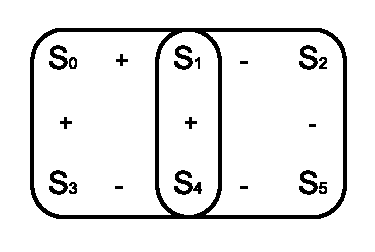
\includegraphics[width=1\textwidth]{pictures/Type2_3x2_2.eps}
		\label{fig:Type2_3x2_2}
	\end{minipage}
	\caption{Системы состоящие из двух плакетов второго типа}
	\label{fig:Type2_32}
%\end{minipage}
%\hspace{40pt}
%\begin{minipage}{0.3\textwidth}
	%\centering
	%\resizebox{100px}{70px}{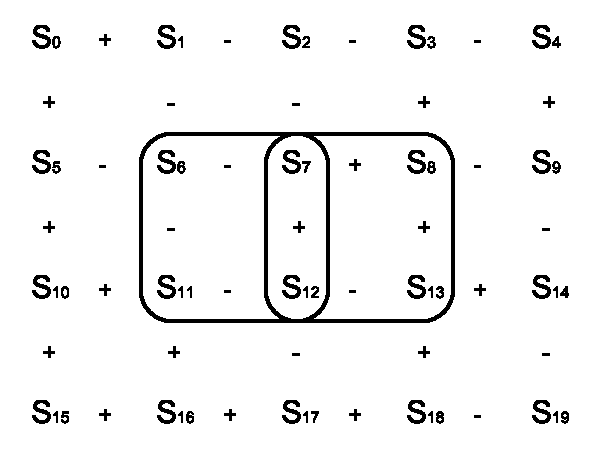
\includegraphics{pictures/Type2_5x4.eps}}
	%\caption{Система из 20 спинов с двумя плакетами 2-го типа в центре}
	%\label{fig:Type2_5x4}
%\end{minipage}
\end{figure}


Легко найти энергию, спиновый избыток и конфигурации основного состояния при известном расположении фрустрированных пар спинов. Энергия и кратность вырождения основного состояния для систем на рисунке \ref{fig:Type2_32} $E_{gs}/N=-0.83$, $g=2$. Спиновый избыток основного состояния $M_{gs}/N=0$ для системы на рисунке \ref{fig:Type2_32}(a) и $M_{gs}/N=\pm 0.33$ на рисунке \ref{fig:Type2_32}(b).

%На рисунке \eqref{fig:Type2_5x4} представлена система из двадцати спинов, в центре которой находятся два плакета 2-го типа, имеющие общую пару спинов. Исходя из предыдущего примера, данная система должна обладать одной фрустрированной парой отмеченной на рисунке. Полный перебор состояний подтверждает, что в данной системе есть два основных состояния ($E_{gs}/N=-1.45$, $M_{gs}=\pm 8$), а фрустрация действительно расположена так, как показано на рисунке \eqref{fig:Type2_5x4}.

На рисунках \ref{fig:4x4.1}(a-d) в центре решетки находится плакет 2-го типа, содержащий фрустрацию. Размещение фрустрации в плакете не 2-го типа приводит к возникновению еще одного возбуждения в нем. В данном примере существует 8 основных состояний ($E_{gs}/N=-1.25$, $g=8$, $M_{gs}/N=\pm 0.25$ - рисунок \ref{fig:4x4.1} (a), $M_{gs}/N=\pm 0.25$ - рисунки \ref{fig:4x4.1} (a,b), $M_{gs}/N=\pm 0.08$ - рисунок \ref{fig:4x4.1} (c), $M_{gs}/N=\pm 0.08$ - рисунок \ref{fig:4x4.1} (d)). Спиновый избыток основного состояния обусловлен соотношением количества ферромагнитных и антиферромагнитных связей. Фрустрации могут изменять это соотношение, потому что фрустрированная антиферромагнитная связь приведет к ферромагнитному упорядочению в паре спинов, и наоборот.

\begin{figure}[H]
	\begin{minipage}[h]{0.2\linewidth}
		\centering(a)
		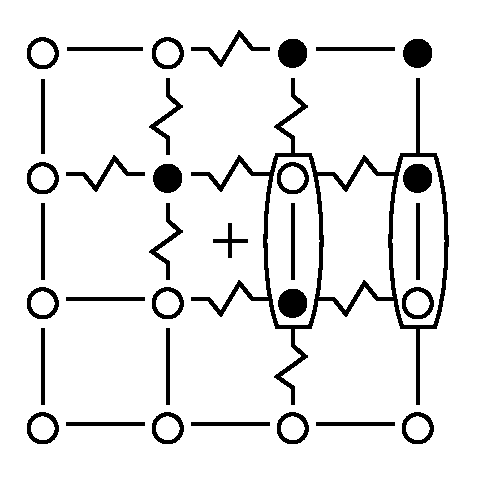
\includegraphics[width=1\linewidth]{pictures/Cl1_Type2_gs1.eps}
	\end{minipage}
	\hfill
	\begin{minipage}[h]{0.2\linewidth}
		\centering(b)
		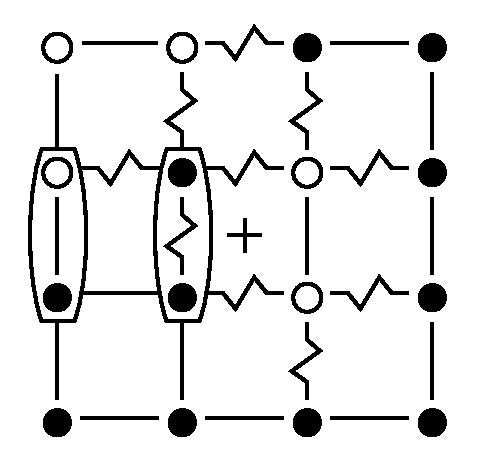
\includegraphics[width=1\linewidth]{pictures/Cl1_Type2_gs2.eps}
	\end{minipage}
	\hfill
	\begin{minipage}[h]{0.2\linewidth}
		\centering(c)
		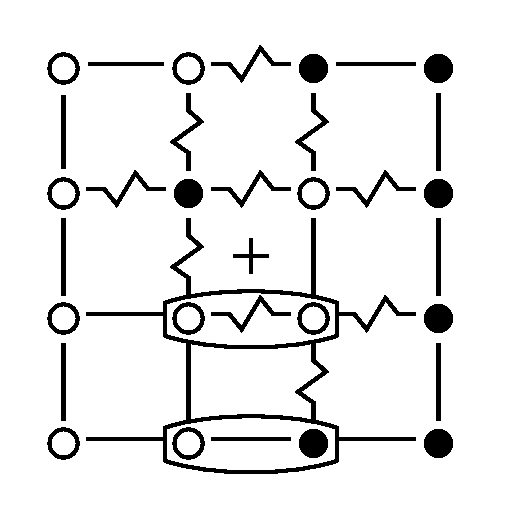
\includegraphics[width=1\linewidth]{pictures/Cl1_Type2_gs3.eps}
	\end{minipage}
	\hfill
	\begin{minipage}[h]{0.2\linewidth}
		\centering(d)
		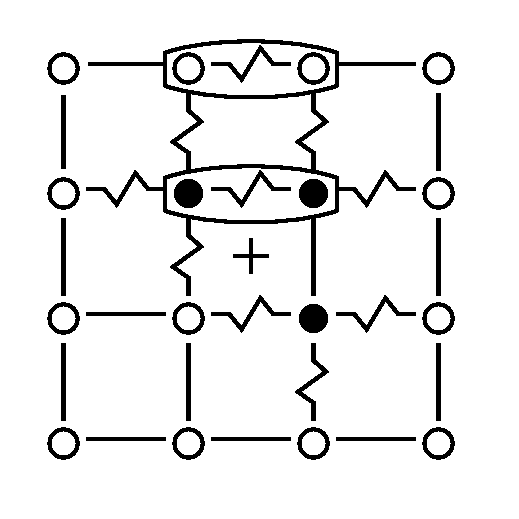
\includegraphics[width=1\linewidth]{pictures/Cl1_Type2_gs4.eps}
	\end{minipage}
	\caption{Основные состояния системы (a, b, c, d). Фрустрированные пары спинов обведены.}
	\label{fig:4x4.1}
	
\end{figure}

Для примера на рисунке \ref{fig:4x7}, $E_{gs}/N=-1.18$, $M_{gs}/N=0$, существует только два основных состояния $g=2$. При этом имеется три фрустрированные пары. Таким образом, наличие фрустраций в основном состоянии не всегда приводит к макроскопическому вырождению. 

\begin{figure}[H]
	\centering
	\resizebox{150px}{75px}{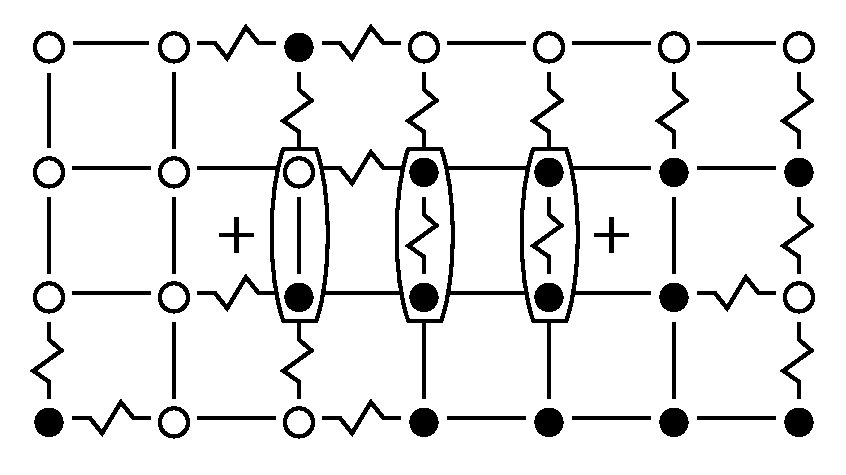
\includegraphics{pictures/Cl7x4_Type2.eps}}
	\caption{Основное состояние решетки с двумя плакетами второго типа}
	\label{fig:4x7}
\end{figure}

На рисунке \ref{fig:5x5.22F} приведен пример ($E_{gs}/N=-1.44$, $g=4$, $M_{gs}/N=\pm 0.11$ для рисунка \ref{fig:4x7} (a) и $M_{gs}=\pm 0.04$ для \ref{fig:4x7} (b)), когда два плакета 2-го типа имеют один общий спин. Несмотря на уменьшение количества фрустрированных пар, по сравнению с предыдущим примером, наблюдается увеличение вырождения основного состояния. Комбинаторика возникает по причине того, что существует несколько вариантов размещения фрустрированных пар на решётке.

\begin{figure}[H]
	\centering
	\begin{minipage}[h]{0.25\linewidth}
		\centering(a)
		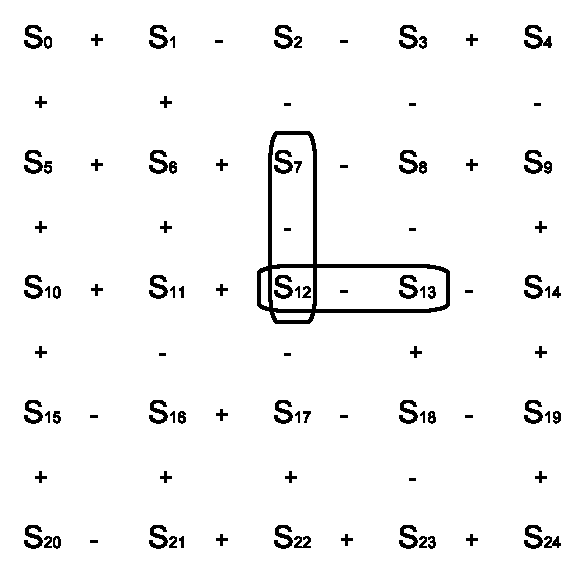
\includegraphics[width=1\linewidth]{pictures/Cl5x5_Type2_gs1.eps}
	\end{minipage}
	\hspace{15pt}
	\begin{minipage}[h]{0.25\linewidth}
		\centering(b)
		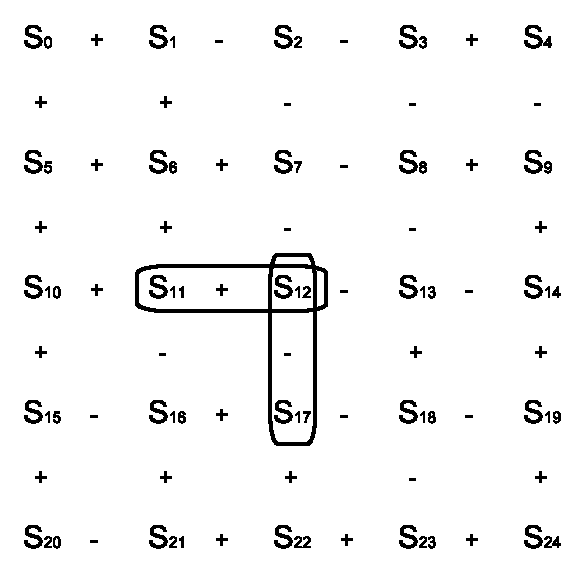
\includegraphics[width=1\linewidth]{pictures/Cl5x5_Type2_gs2.eps}
	\end{minipage}
	\caption{Основные состояния решетки с двумя плакетами второго типа}
	\label{fig:5x5.22F}
\end{figure}

На основе рассмотренных примеров можно сделать несколько выводов:

\begin{enumerate}
	\item Плакеты 2-го типа являются единственной причиной возникновения фрустраций в основном состоянии.
	\item В основном состоянии фрустрации расположены между плакетами 2-го типа или между плакетом и краем решётки в зависимости от расстояний.
	\item Макроскопическое вырождение основного состояния обусловлено альтернативными вариантами размещения фрустраций.
\end{enumerate}

\section{Природа вырождения основного состояния}

Можно вычислить все основные состояния путём попарного комбинирования плакетов 2-го типа. Рассмотрим работу алгоритма на примере решётки состоящей из 64 спинов \ref{fig:12PS_cell64_J72_5} (a).

\begin{figure}[H]
	\centering
	\begin{minipage}[h]{0.3\linewidth}
		\centering(a)
		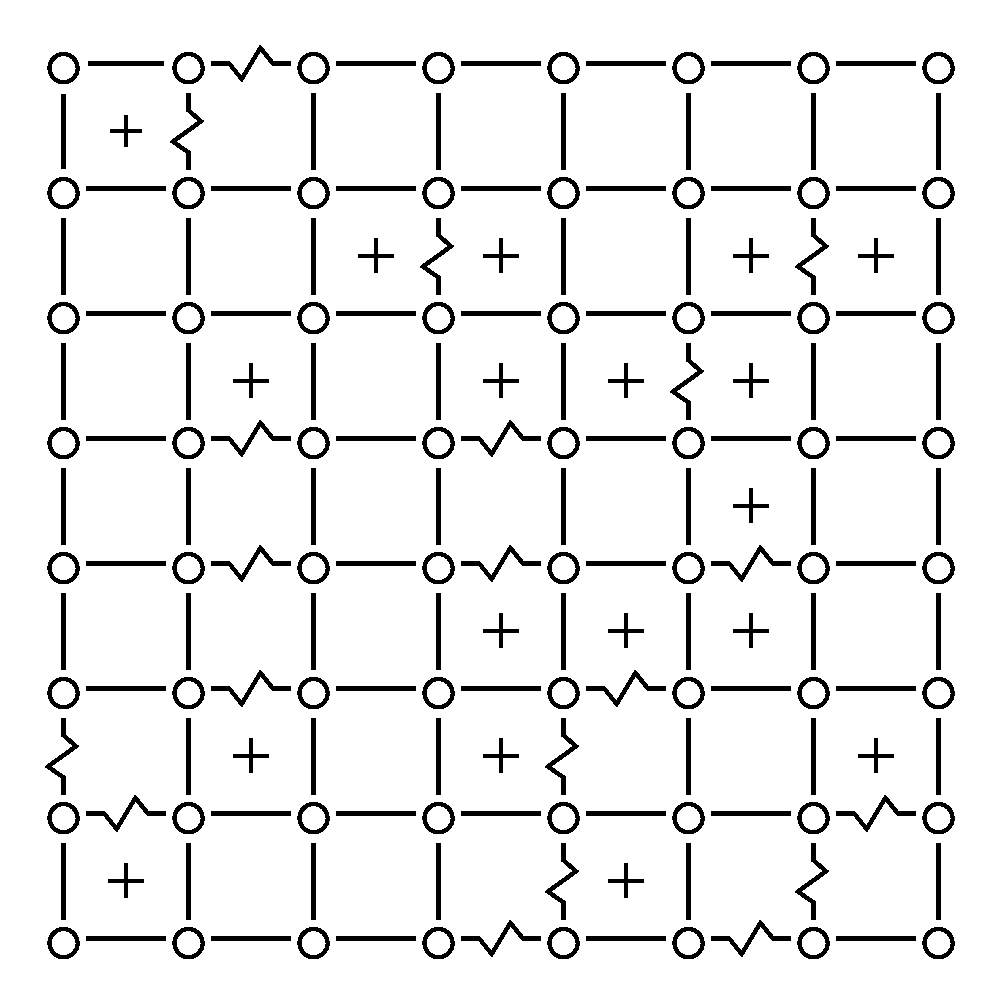
\includegraphics[width=1\linewidth]{pictures/cell64_J72_5.eps}
	\end{minipage}
	\hspace{10pt}
	\begin{minipage}[h]{0.3\linewidth}
		\centering(b)
		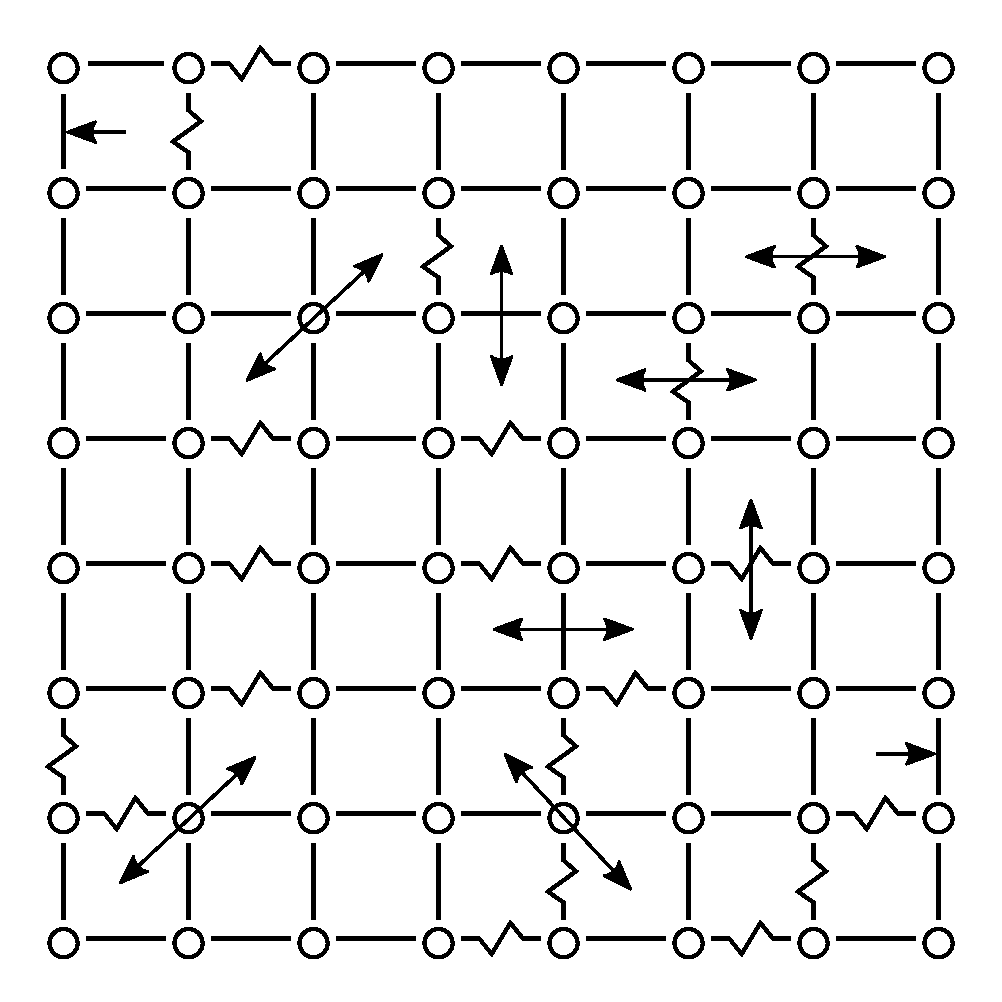
\includegraphics[width=1\linewidth]{pictures/1PS_cell64_J72_5.eps}
	\end{minipage}
	\hspace{10pt}
	\begin{minipage}[h]{0.3\linewidth}
		\centering(c)
		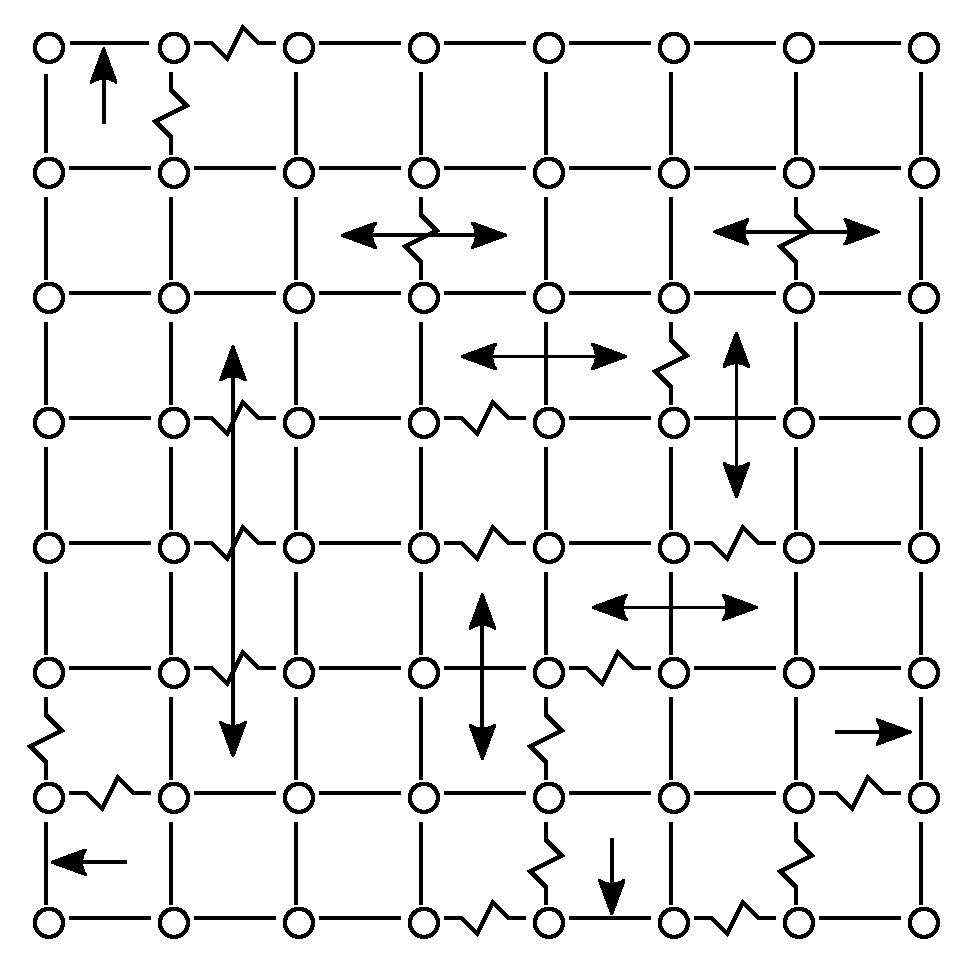
\includegraphics[width=1\linewidth]{pictures/2PS_cell64_J72_5.eps}
	\end{minipage}
	\caption{(a) - пример решетки 64 спина, (b,c) - комбинации плакетов 2-го типа, обладающих минимальным числом фрустраций}
	\label{fig:12PS_cell64_J72_5}
\end{figure}


Сначала каждому плакету присваиваются координаты $x$ и $y$. Далее происходит комбинирование разбиений плакетов второго типа по парам. Рассматриваются случаи, когда фрустрации возникают между каждой парой плакетов и когда размещение возбуждений происходит между плакетом и краем решётки. Число фрустраций между $i,j$-той парой плакетов определяется как $\left|x_i-x_j\right|+\left|y_i-y_j\right|$,  число фрустраций, возникающее от плакета 2-го типа до ближайшего края решетки определяется как $R_{ij}+1$, где i - номер плакета 2-го типа, j - номер ближайшего плакета находящегося на краю решётки, $R_{ij}$ - расстояние между ними. После перебора всех пар плакетов 2-го типа рассматриваются комбинации, которые по подсчётам обладают минимальным числом фрустраций. Две из них представлены на рисунке \ref{fig:12PS_cell64_J72_5} (b,c).

На основании полученных комбинаций пары спинов, находящиеся между плакетами, отмечаются как фрустрированные (рис. \ref{fig:12F_cell64_J72_5}).

\begin{figure}[H]
	\centering
	\begin{minipage}[h]{0.3\linewidth}
		\centering(a)
		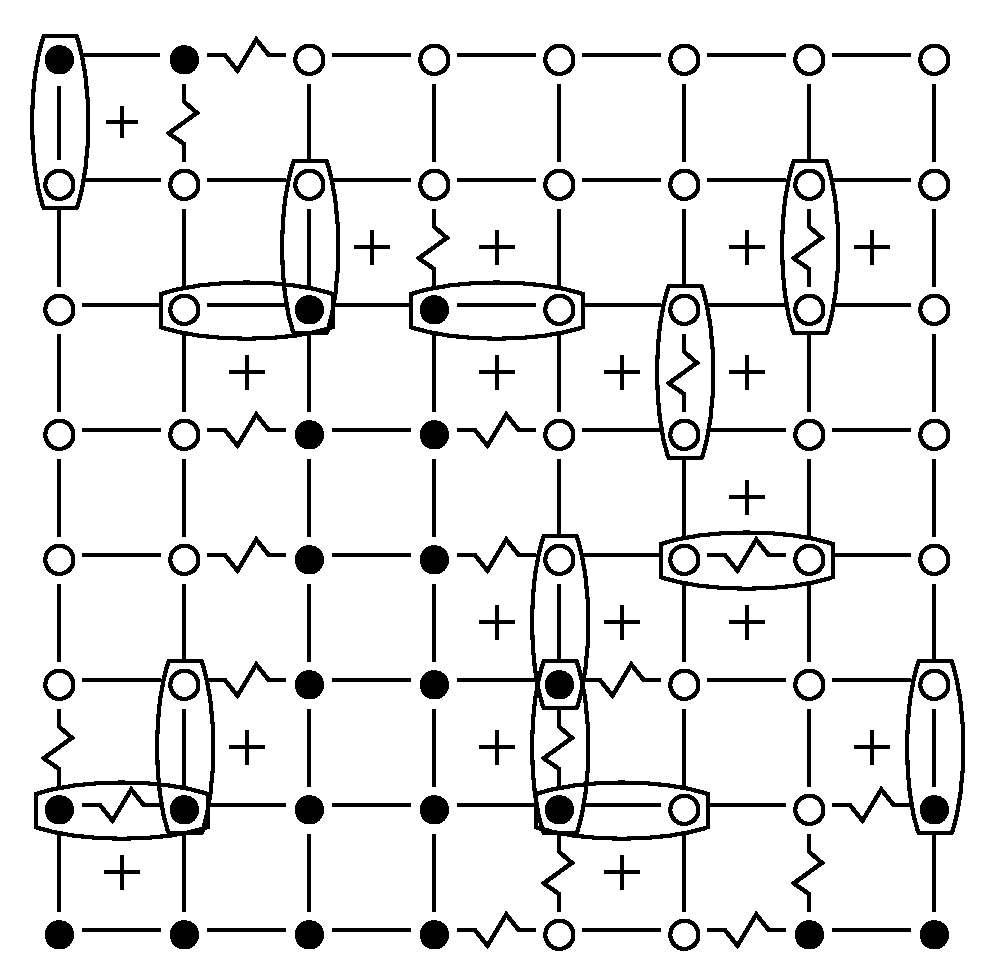
\includegraphics[width=1\linewidth]{pictures/1Conf_cell64_J72_5.eps}
	\end{minipage}
	\hspace{15pt}
	\begin{minipage}[h]{0.3\linewidth}
		\centering(b)
		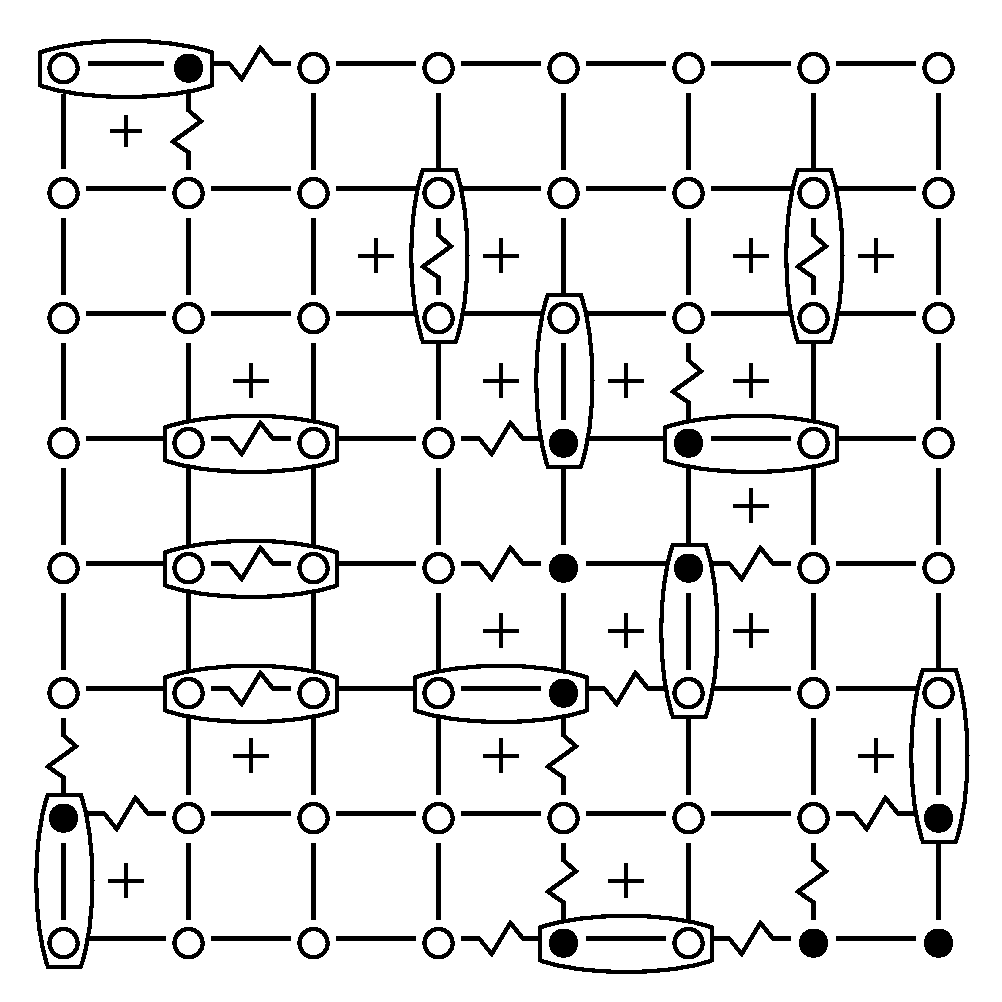
\includegraphics[width=1\linewidth]{pictures/2Conf_cell64_J72_5.eps}
	\end{minipage}
	\caption{Основные состояния решетки \ref{fig:12PS_cell64_J72_5} (a)}
	\label{fig:12F_cell64_J72_5}
\end{figure}

Всего для данной решётки было получено $g=124$ основных состояния с энергией $E_{gs}/N=-1.34$ и спиновым избытком $M_{gs}/N$ от $\pm 0.28$ до $\pm 0.66$. Данное решение полностью совпадает с результатами, полученными с помощью алгоритма \ref{alg:addititional_algorithm}.

Таким образом, высокая кратность вырождения основного состояния обусловлена несколькими причинами:

1. Различные комбинации плакетов 2-го типа могут давать одинаковое количество фрустраций, как показано в предыдущем примере на рисунках \ref{fig:12PS_cell64_J72_5} (b,c).

2. Может существовать несколько вариантов размещения фрустраций между плакетами, если их координаты $x,y$ различаются (рис. \ref{fig:5x5.22F}).

3. Выбор граничных условий может влиять на вырождение. Например в случает размещения фрустрированного плакета рядом с двумя границами приводит к увеличению вариантов размещения фрустраций (рис. \ref{fig:4x4.1}).



\section{Решение исчерпывающим перечислением}

Для исследования быр разработан алгоритм исчерпывающего перечисления.

Модель спинового стекла Эдвардса-Андерсона представляет собой плоскую решетку Изинга:

\begin{equation}
	E = -\sum J_{ij} S_i S_j + h \sum S_i.
	\label{eq:ising_energy}
\end{equation}
Это приводит к конкурирующим антиферромагнитным (при $J_{ij}=-1$) и ферромагнитным (при $J_{ij}=+1$) взаимодействиям. В нашей модели энергия обменного взаимодействия не зависит от расстояния между взаимодействующими спинами. Однако, знакопеременный характер обменных интегралов $J_{ij}$ может быть связан с искажениями в размещении взаимодействующих атомов на решетке, осцилляциями электронной плотности.

Рассмотрим одномерную цепочку из трёх спинов ($L=3$), взаимодействующих ферромагнитно. Таким образом, все $J_{ij}=+1$.  Обозначим $\beta = (kT)^{-1}$.  Статистическая сумма принимает вид:

\begin{equation}
	Z_3 = e^{3\beta - 3\beta h} + 3e^{\beta - h - \beta} + 3e^{\beta h - \beta} + e^{3\beta + 3\beta h}.
	\label{eq:stat_3}
\end{equation}

Присоединим вторую цепочку параллельно первой. С учетом того, что у нас все взаимодействия ферромагнитные

\begin{equation}
	\label{eq:stat_3_un}
	\begin{alignedat}{2}
		Z_6 = Z_3 e^{\beta  h-\beta }+Z_3 e^{\beta  h-\beta }+Z_3 e^{\beta  h-\beta }+Z_3 e^{3 \beta +3 \beta  h}+ \\
		Z_3 e^{\beta  (-h)-\beta }+Z_3 e^{\beta  (-h)-\beta }+Z_3 e^{\beta  (-h)-\beta }+Z_3 e^{3 \beta -3 \beta  h}.
	\end{alignedat}
\end{equation}

В результате получаем статистическую сумму для решетки $3 \times 2$:

\begin{equation}
	\label{eq:stat_3_res}
	\begin{alignedat}{2}
		Z_6 = 6 e^{-5 \beta }+12 e^{-\beta }+2 e^{3 \beta }+e^{9 \beta -6 \beta  h}+6 e^{3 \beta -4 \beta  h}+6 e^{-3 \beta -2 \beta  h}+\\
		9 e^{\beta -2 \beta  h}+6 e^{2 \beta  h-3 \beta }+9 e^{\beta +2 \beta  h}+6 e^{3 \beta +4 \beta  h}+e^{9 \beta +6 \beta  h}.
	\end{alignedat}
\end{equation}

Алгоритм численного расчета  параметров статистической суммы (плотности состояний, вырождения или энтропии, энергии и спинового избытка состояний) тогда выглядит следующим образом \ref{alg:addititional_algorithm}:


\begin{algorithm}[H]
	\textbf{ВХОД:} Размер и геометрия решетки (количество и координаты спинов, граничные условия, число соседей), распределение обменных констант.\\
	\textbf{ВЫХОД:} Параметры статистической суммы, плотность состояний - (вырождение или энтропия, энергия и спиновый избыток).
	\begin{algorithmic}
		\STATE {Рассчитать плотность состояний для первой 1D цепочки}
		\FOR {Количество слоев в решетке\\}
		{
			\STATE {Рассчитать плотность состояний для присоединяемой 1D цепочки}
			\FOR {длина 1D цепи\\}
			{
				\STATE {Рассчитать плотность состояний для получившейся решетки}
			}
			\ENDFOR\\
		}
		\ENDFOR
	\end{algorithmic}
	\caption{Вычисление параметров статистической суммы методом присоединения 1D цепочек.}
	\label{alg:addititional_algorithm}
\end{algorithm}

В результате для квадратной решетки $L \times L=N$ сложность алгоритма полного перебора падает с $2^{N}$ до $L \cdot 2^L + (L - 1) \cdot 2^L$. Таким образом прирост производительности для решетки из 9-ти спинов составляет примерно 92\% и на 27 порядков для системы из 100 спинов.


\section{Энергия основного состояния}

Результаты решения задачи о вычислении энергии основного состояния спинового стекла в модели Эдвардса-Андерсона приведены в таблице \ref{tab:Egs}. Из таблицы видно, что значения энергий основного состояния  имеют большой разброс.

\begin{table}[h]
	\begin{tabular}{|l|c|l|}
		\hline
		Method                                   & $E_{gs}$                                       & ссылка                                          \\ \hline
		Thouless-Anderson-Palmer (TAP) Approach & 0                                              & \cite{thouless1977solution}    \\ \hline
		Replica Method                            & $-2/\pi$                                       & \cite{sherrington1975solvable} \\ \hline
		Partition function                      & -0.5                                           & \cite{tanaka1980analytic}      \\ \hline
		Mean random field                       & $-1/\sqrt{2\pi}$                               & \cite{klein1976comparison}     \\ \hline
		Monte-Carlo                             & -0.76                                          & \cite{kirkpatrick1978infinite} \\ \hline
		Algorithm of Shraudorphs-Kamensky        & -1.33                                          & \cite{karandashev2019global}   \\ \hline
		Parallel Tempering   & -1.40193                                       & \cite{palmer1999ground}        \\ \hline
		Branch-and-Cut Algorithm              & -1.40197                         
		& \cite{campbell2004energy}      \\ \hline
		
		Parallel tempering Monte-Carlo  & -1.31479                                       & \cite{roma2009ground}          \\ \hline
		
		
		
	\end{tabular}
	\caption{Удельная энергия основного состояния}
	\label{tab:Egs}
\end{table}

Мы вычислили значение энергии основного состояния в модели Эдвардса-Андерсона точно с помощью исчерпывающего перечисления (алгоритм \ref{alg:addititional_algorithm}). На графике \ref{fig:E(Q)} представлена зависимость удельной энергии основного состояния $E_{gs}/N$ от числа плакетов второго типа $Q$. 
%и с помощью описанного выше подхода. Для исследования основных состояний были взяты 2000 различных решёток спинового стекла. Линейный размер $L$ в образцах был от 8 до 32.
%Для каждого размера рассматривались системы с различным чётным $Q$ количеством плакетов 2-го типа от 2 до 16, и для каждого количества плакетов было взято по 10 систем со случайной расстановкой плакетов 2-го типа внутри системы. %Для исследования не  брались решётки с нечётным количеством плакетов 2-го типа так как тогда невозможно добиться одинакового количества отрицательных и положительных обменных интегралов в системе. 

%Из графика \ref{fig:Egs_N_F} видно, что энергия основного состояния системы на один спин увеличивается с числом фрустрированных плакетов. Диапазон таких значений составляет -1.92578 ; -1.34375. Более низкое значение удельной энергии по сравнению с данными в таблице \ref{tab:Egs} обусловлено тем, что для данного исследования были взяты системы с небольшим количеством плакетов 2-го типа, что уменьшает количество фрустраций в основных состояниях.

\begin{figure}[H]
	\centering
		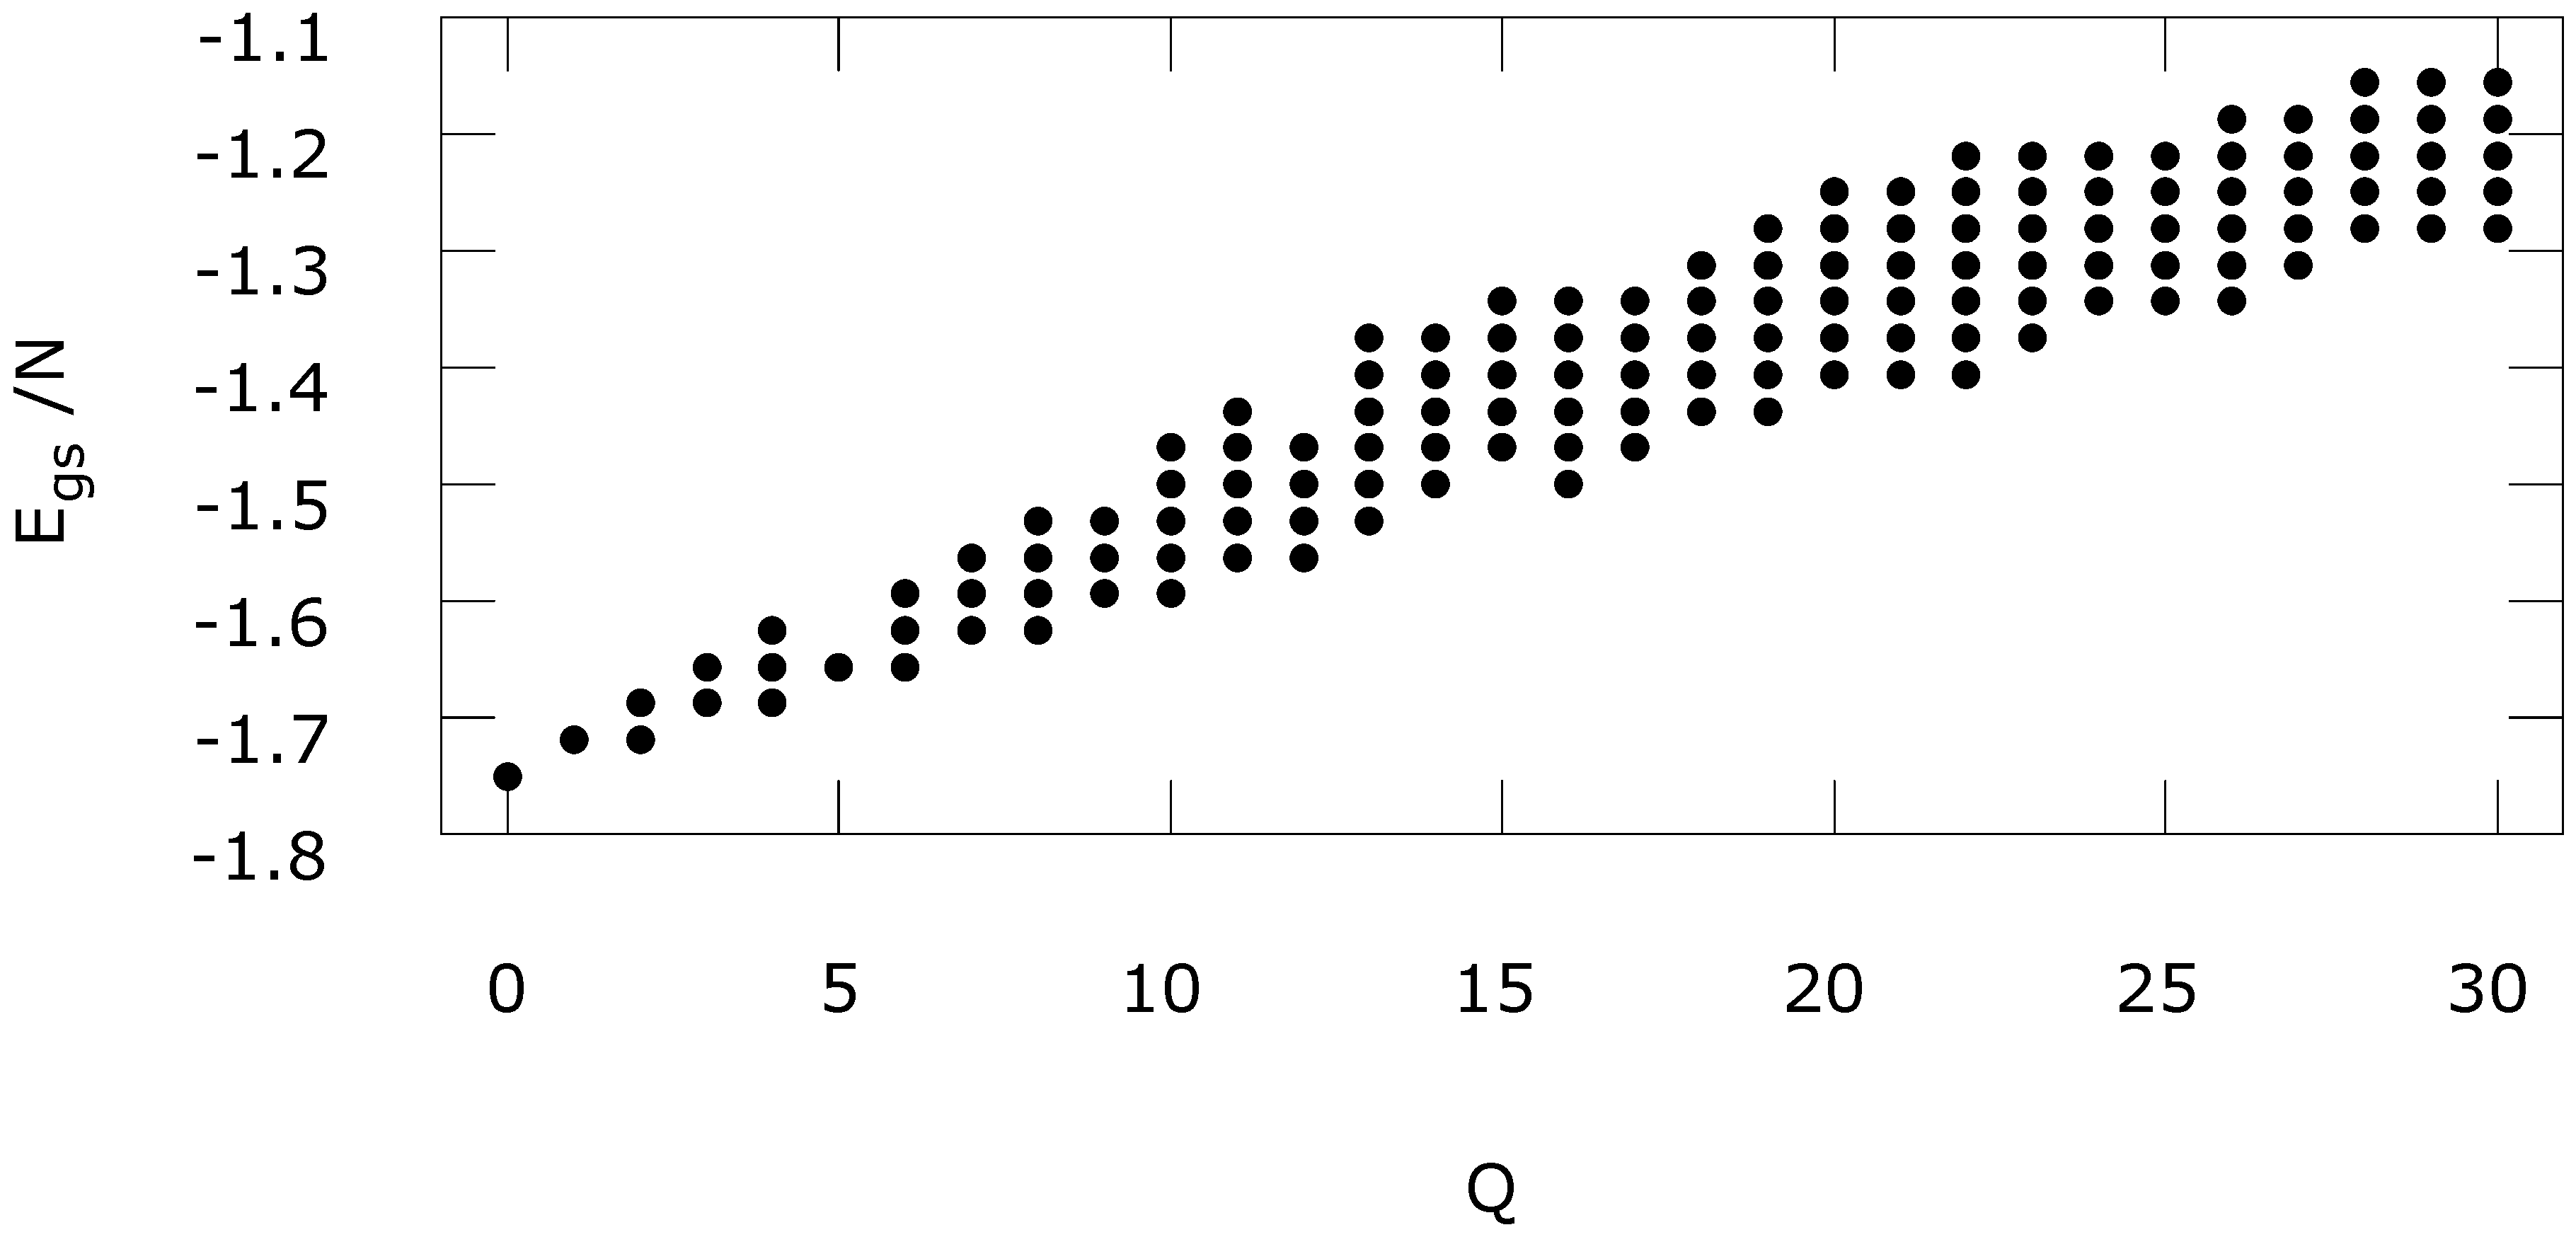
\includegraphics[width=0.5\linewidth]{pictures/E_Q.eps}
	\caption{Энергия основного состояния в зависимости от числа плакетов 2-го типа для $N=64$}
	\label{fig:E(Q)}
\end{figure}

С увеличением количества плакетов 2-го типа $Q$ энергия основного состояния увеличивается в среднем. На скорость увеличения энергии влияет не только количество плакетов 2-го типа, но и их расположение на решетке. Этим объясняется разброс значений энергий основного состояния на рисунке \ref{fig:E(Q)} и в таблице \ref{tab:Egs}.
Увеличение значения энергии основного состояния обусловлено ростом количества фрустраций с увеличением числа плакетов 2-го типа.

\begin{figure}[H]
	\centering
	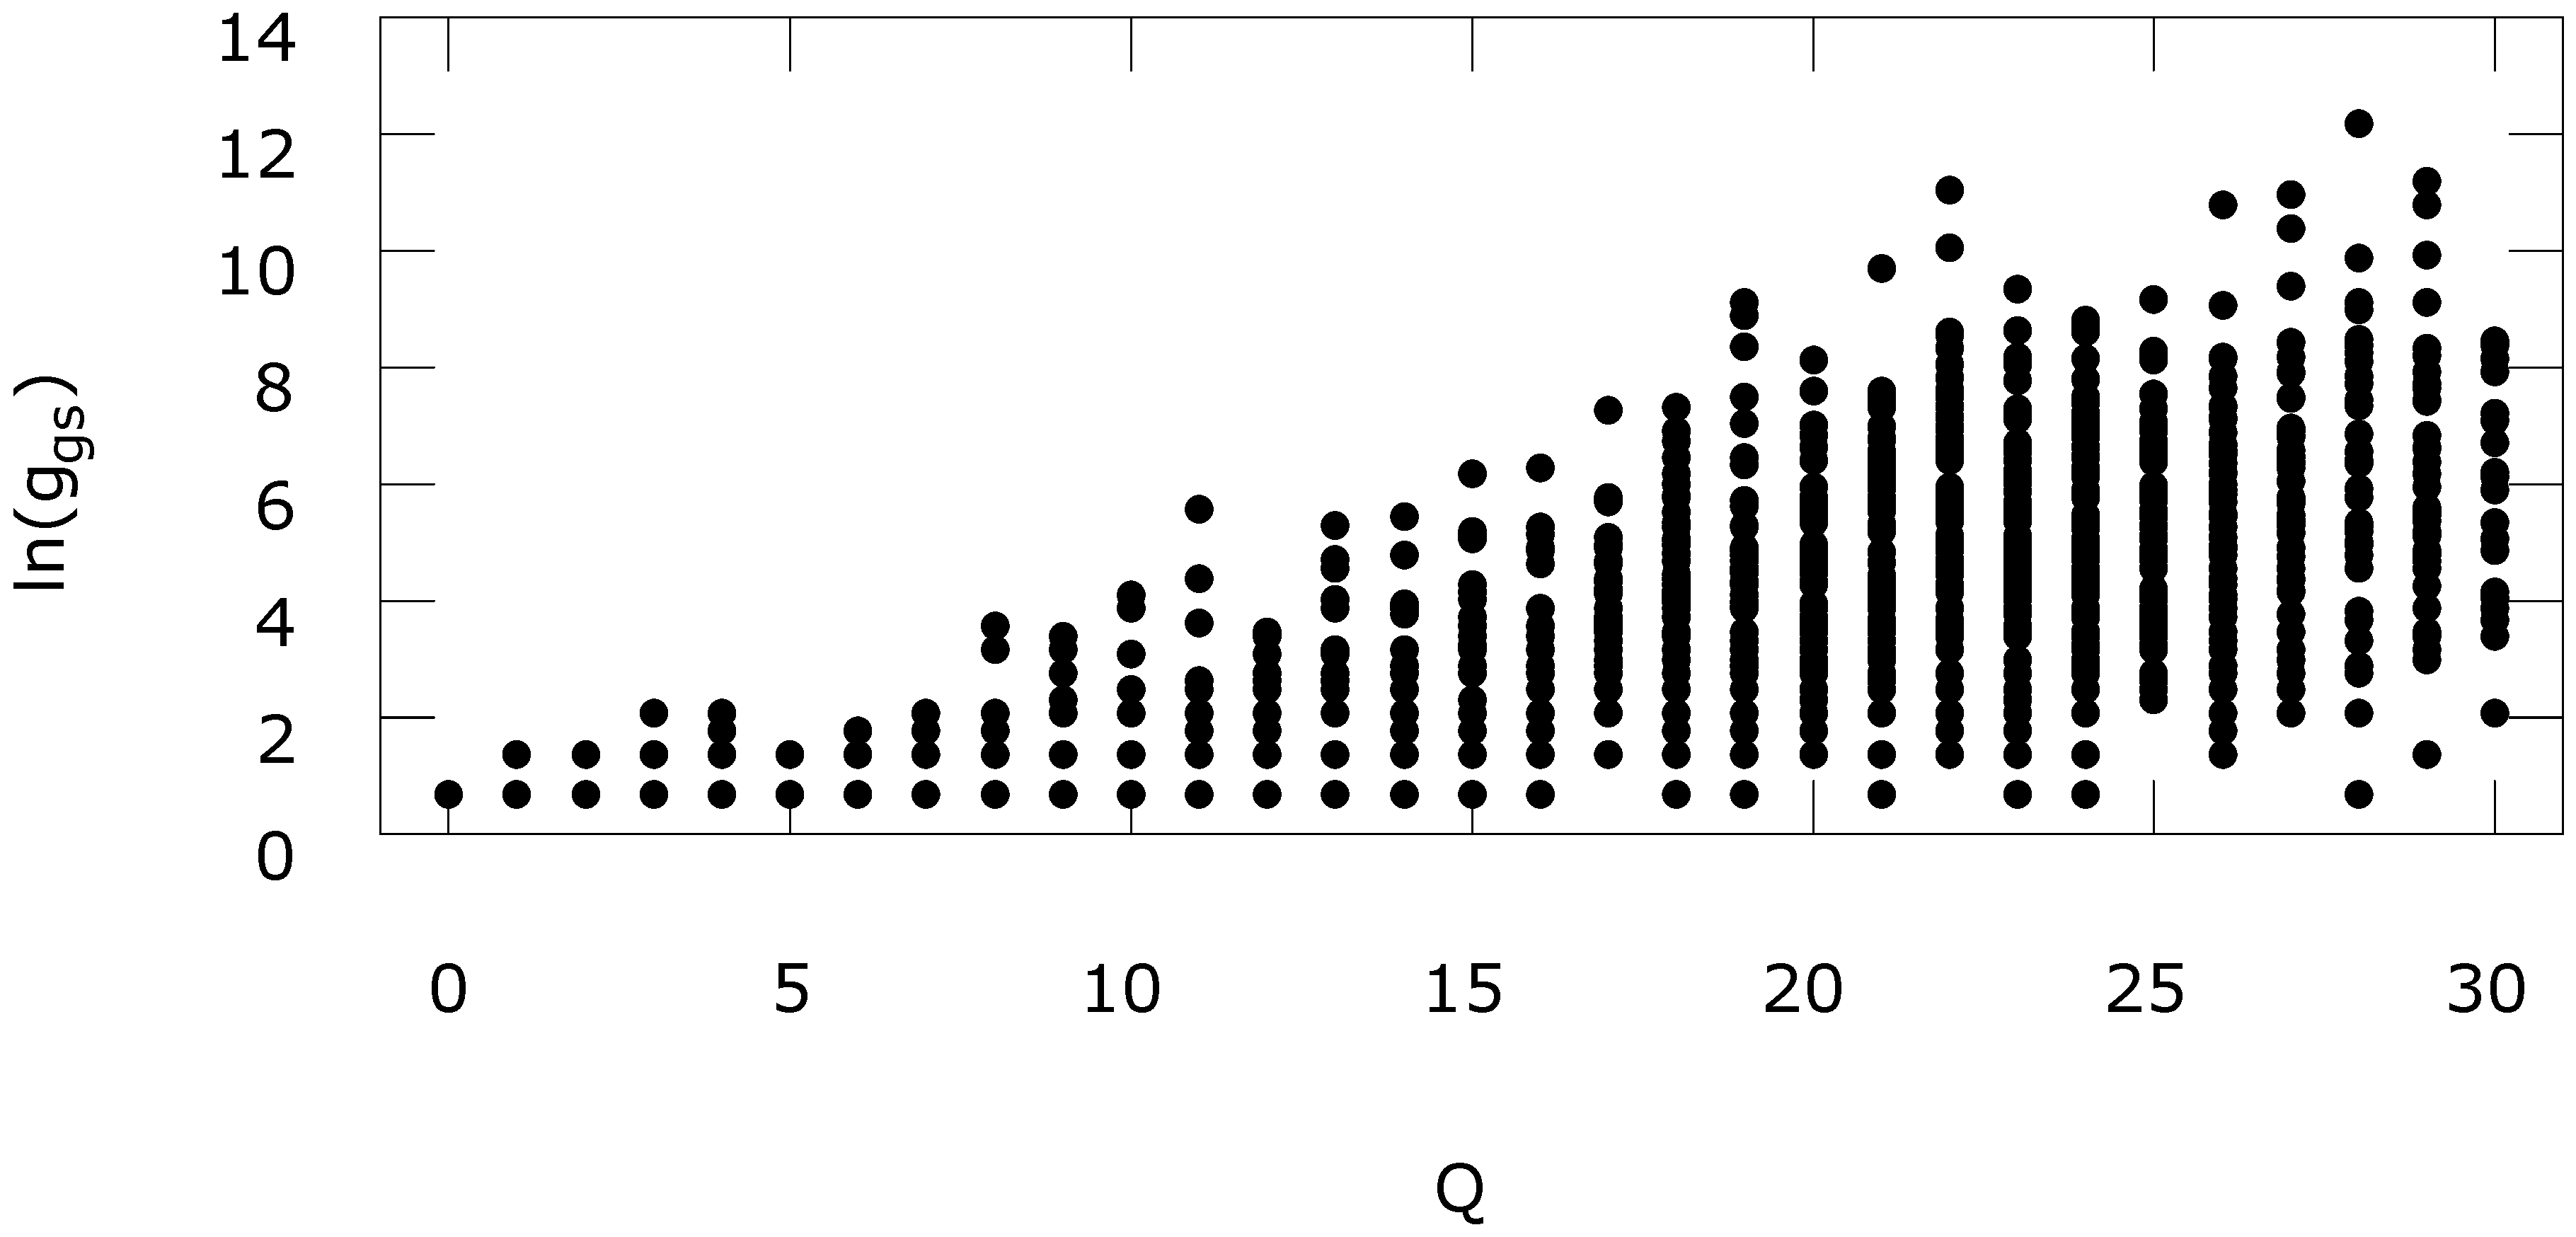
\includegraphics[width=0.5\linewidth]{pictures/g_Q.eps}
	\caption{Вырождение основного состояния в зависимости от числа плакетов 2-го типа для $N=64$}
	\label{fig:g(Q)}
\end{figure}

Увеличение числа плакетов 2-го типа и связанное с ним увеличение количества фрустраций в большинстве случаев ведет к увеличению вырождения основных состояний. Но для некоторых образцов увеличение количества фрустраций не вызывает рост вырождения основного состояния (см. точки с наименьшим значением $g_{gs}=2$ на рис. \ref{fig:g(Q)}). 

\section{Основное состояние во внешнем магнитном поле}

В таблице \ref{tab:Egs} приведены значения энергии основного состояния спинового стекла. На рисунке (\ref{fig:cell_SI_SG_64}) представлены случаи спинового льда и спинового стекла, которые отличаются упорядоченным или неупорядоченным распределением обменных констант. Вычисления показывают, что энергия основного состояния на один спин при $P_+ = 0.5$ и отсутствии воздействия внешнего магнитного поля для моделей спинового льда составила -1.75 и -0.97 (рис. \ref{fig:cell_SI_SG_64}(a) и \ref{fig:cell_SI_SG_64}(c), соответственно), при этом удельная энергия основного состояния спинового стекла в модели Эдвардса-Андерсона составила -1.28. Под спиновым льдом обычно понимается магнетик с периодичностью в обменных ферромагнитных и антиферромагнитных взаимодействиях \cite{peretyatko2017interplay, otsuka2018husimi, andriushchenko2019large, shevchenko2017effect, kato2022flux}. 

\begin{figure}[H]
	\begin{minipage}[h]{0.3\linewidth}
		\centering(a)
		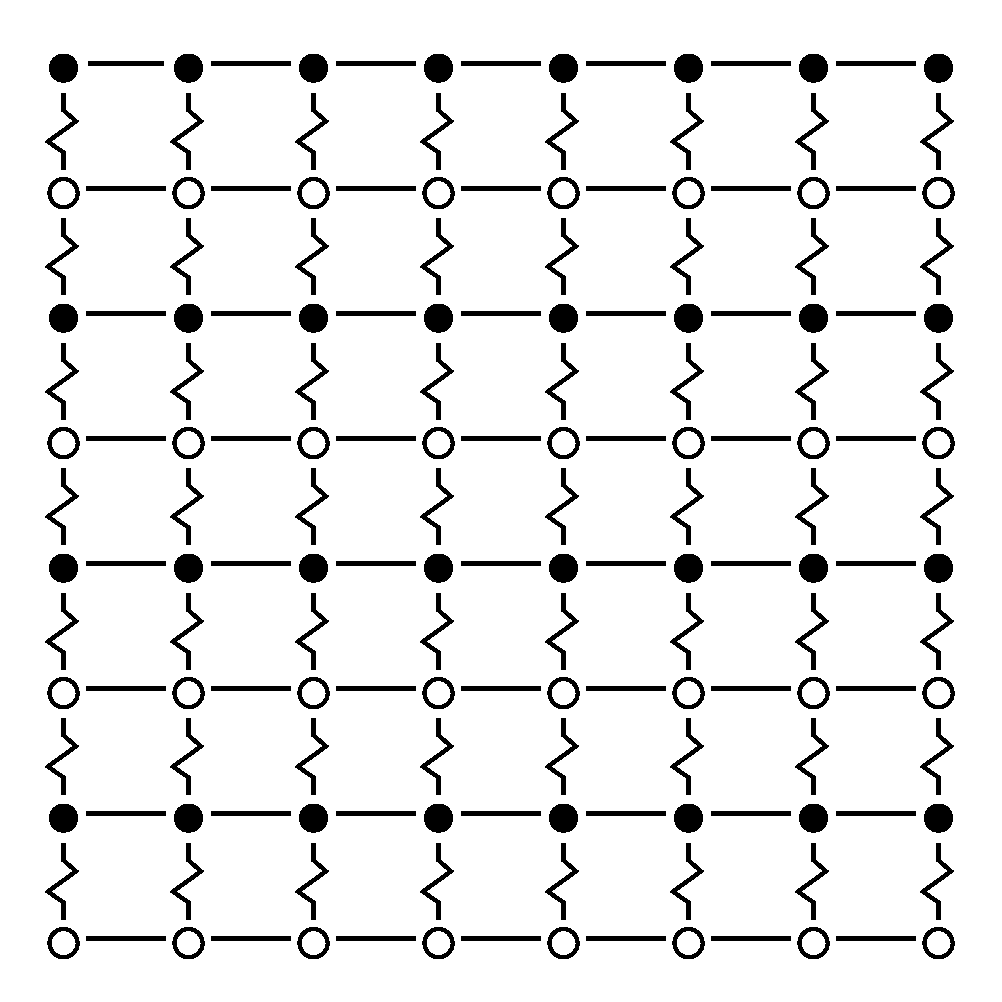
\includegraphics[width=1\linewidth]{pictures/SI_64_J0_1}
	\end{minipage}
	\hfill
	\begin{minipage}[h]{0.3\linewidth}
	\centering(b)
	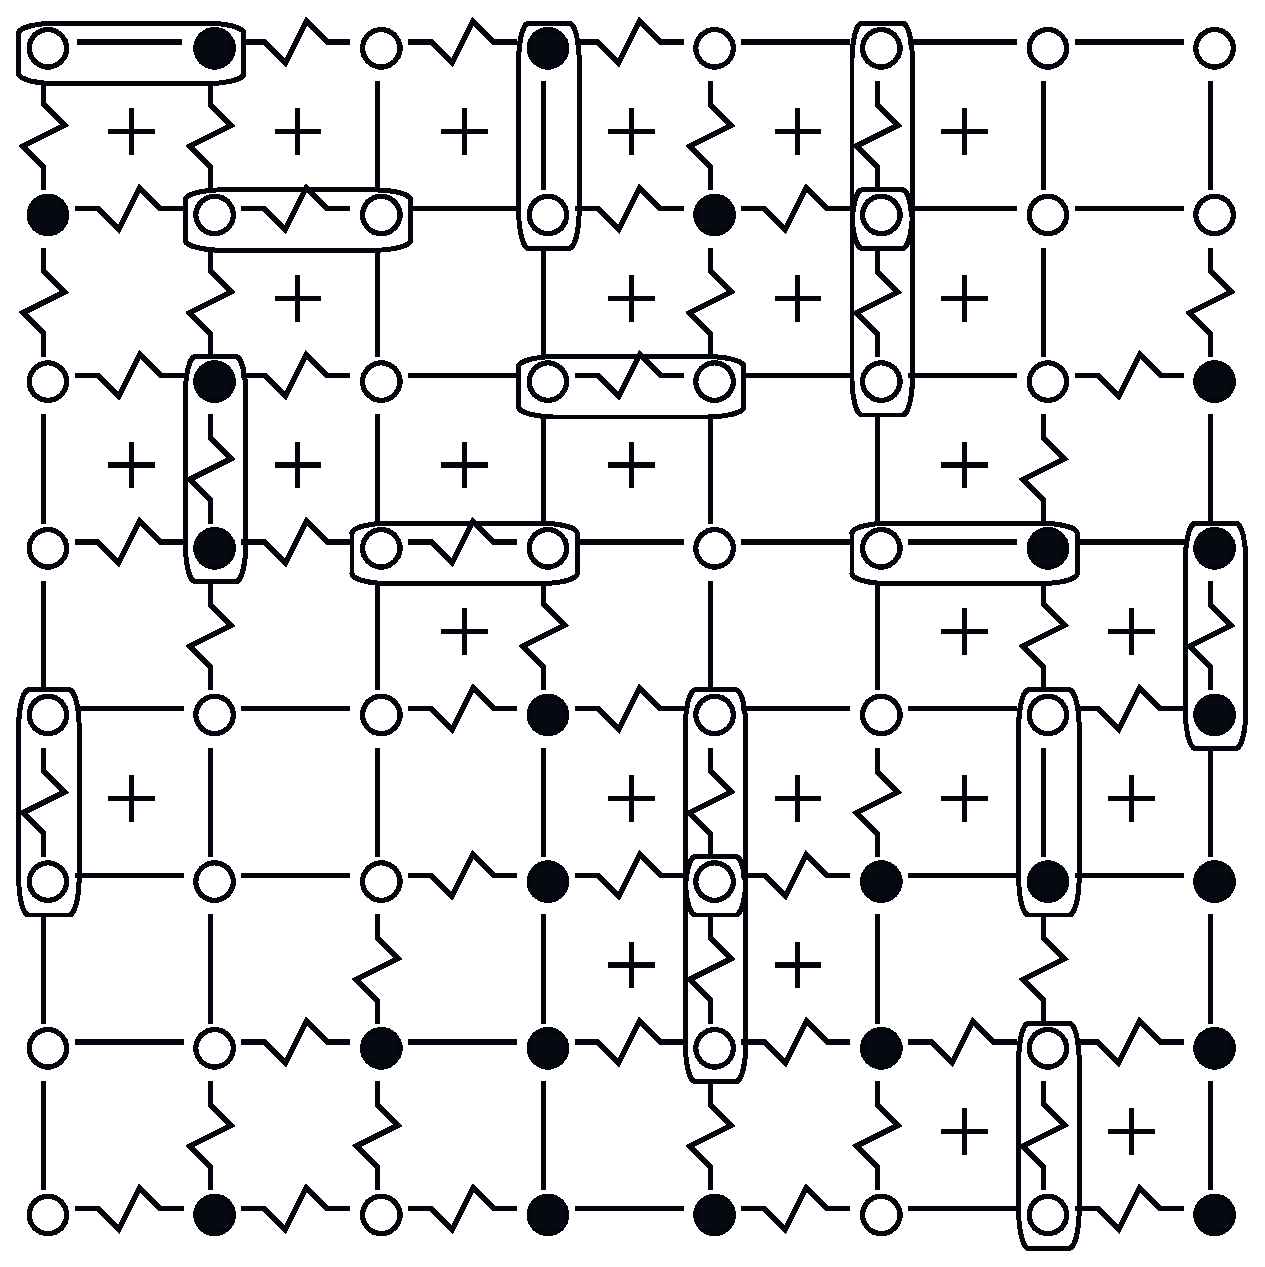
\includegraphics[width=1\linewidth]{pictures/SG_64_J0}
	\end{minipage}
	\hfill
	\begin{minipage}[h]{0.3\linewidth}
		\centering(c)
		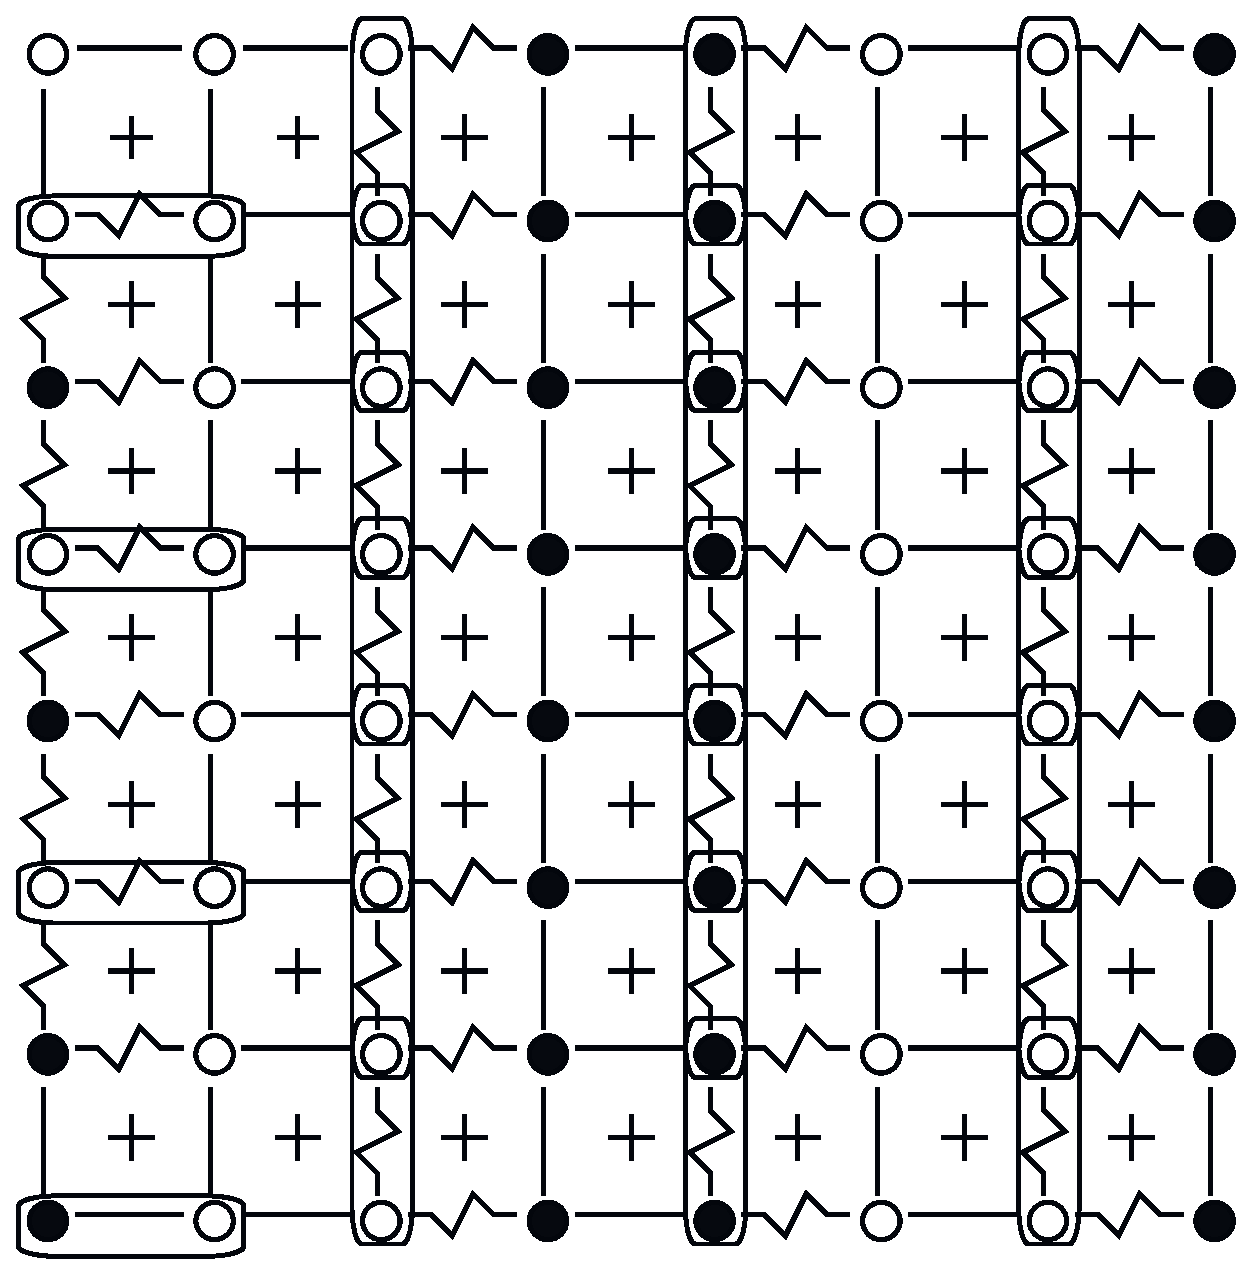
\includegraphics[width=1\linewidth]{pictures/SI_64_J0}
	\end{minipage}
	\hfill
	\caption{Спиновый лед (a,c) и спиновое стекло (b), 64 спина, $P_+ = 0.5$}
	\label{fig:cell_SI_SG_64}

\end{figure}


На рисунке \ref{fig:cell_SI_SG_64}(a) представлена плоская решетка спинового льда, составленная из плакетов 1-го типа, в которой полностью отсутствуют фрустрации. 
На рисунке \ref{fig:cell_SI_SG_64}(b) представлена решетка спинового стекла, в которой из 49 плакетов имеется 16 плакетов 1-го типа, 27 - 2-го типа и 6 плакетов 3-го типа, 15 фрустраций.
В решетке спинового льда на рисунке \ref{fig:cell_SI_SG_64}(c) максимальное количество фрустраций, в данном примере, достигается путем заполнения системы плакетами 2-го типа. Всего 25 фрустраций на 49 плакетов.


\begin{figure}[H]
	\begin{minipage}[h]{0.32\linewidth}
		\centering(a)
		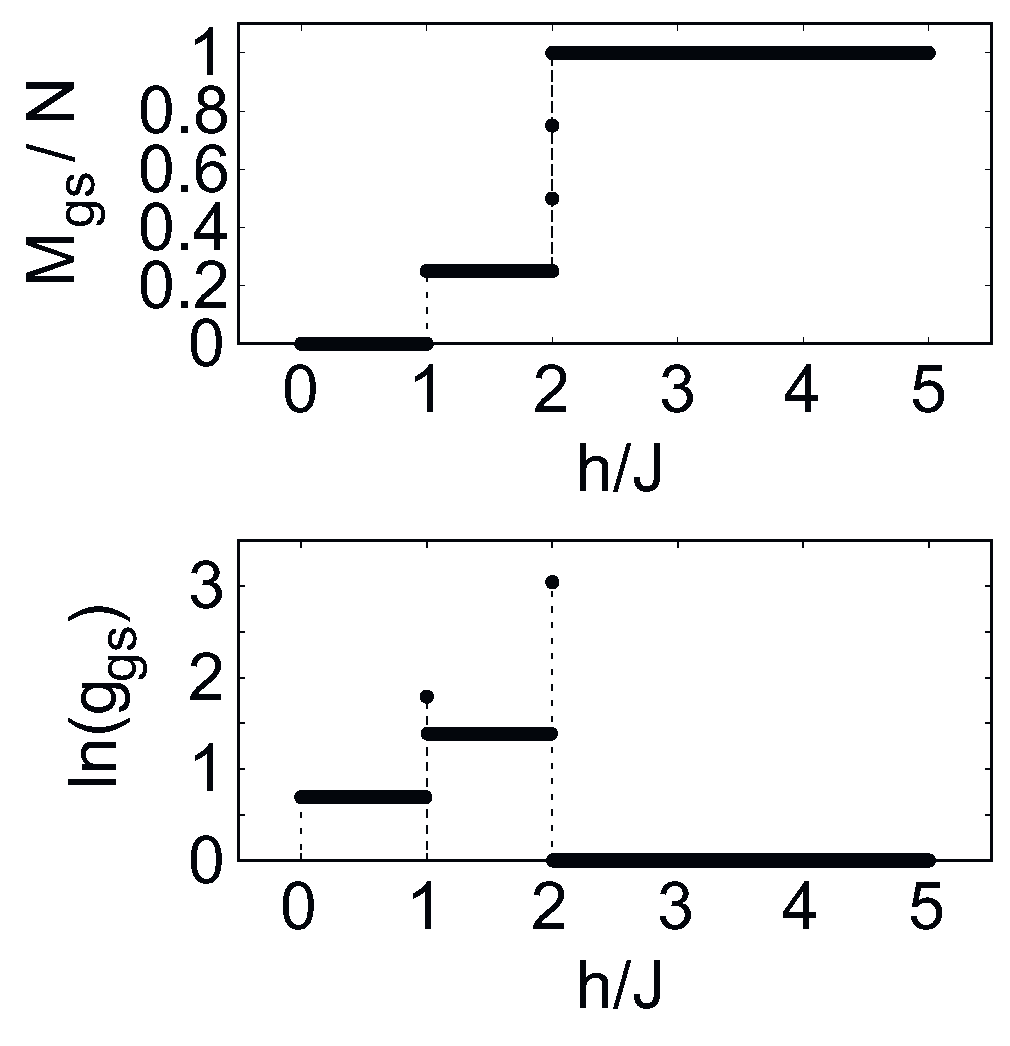
\includegraphics[width=1\linewidth]{pictures/_multiplot_SI64_J0_1}
	\end{minipage}
	\hfill
	\begin{minipage}[h]{0.32\linewidth}
		\centering(b)
		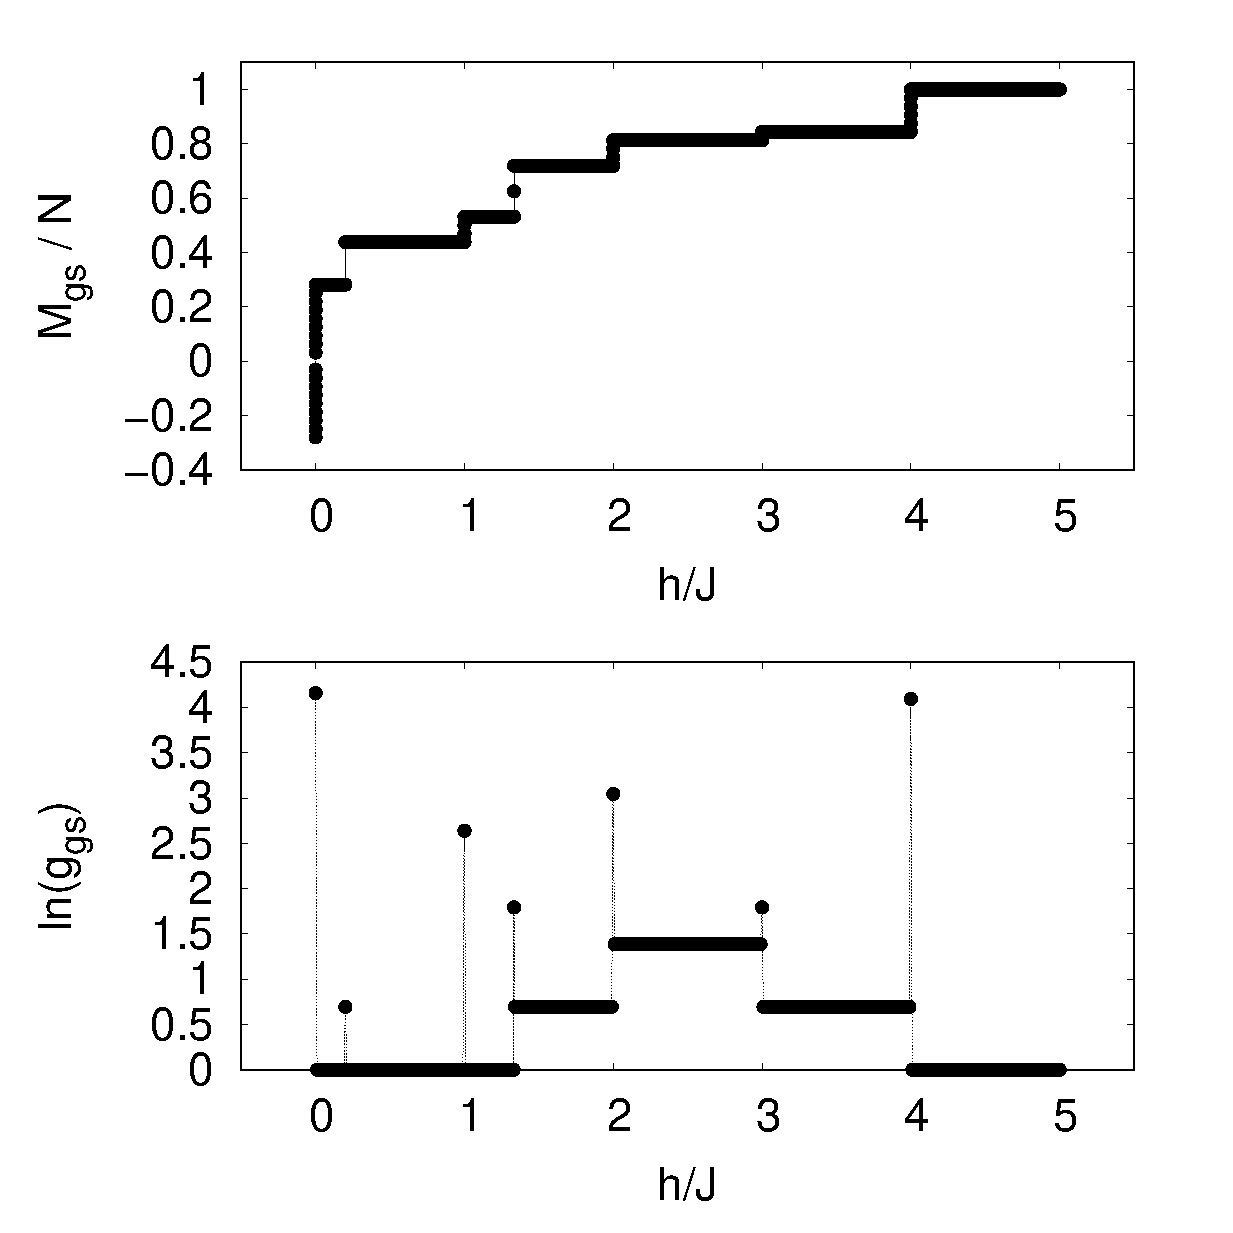
\includegraphics[width=1\linewidth]{pictures/_multiplot_SG64_J0}
	\end{minipage}
	\hfill
	\begin{minipage}[h]{0.32\linewidth}
		\centering(c)
		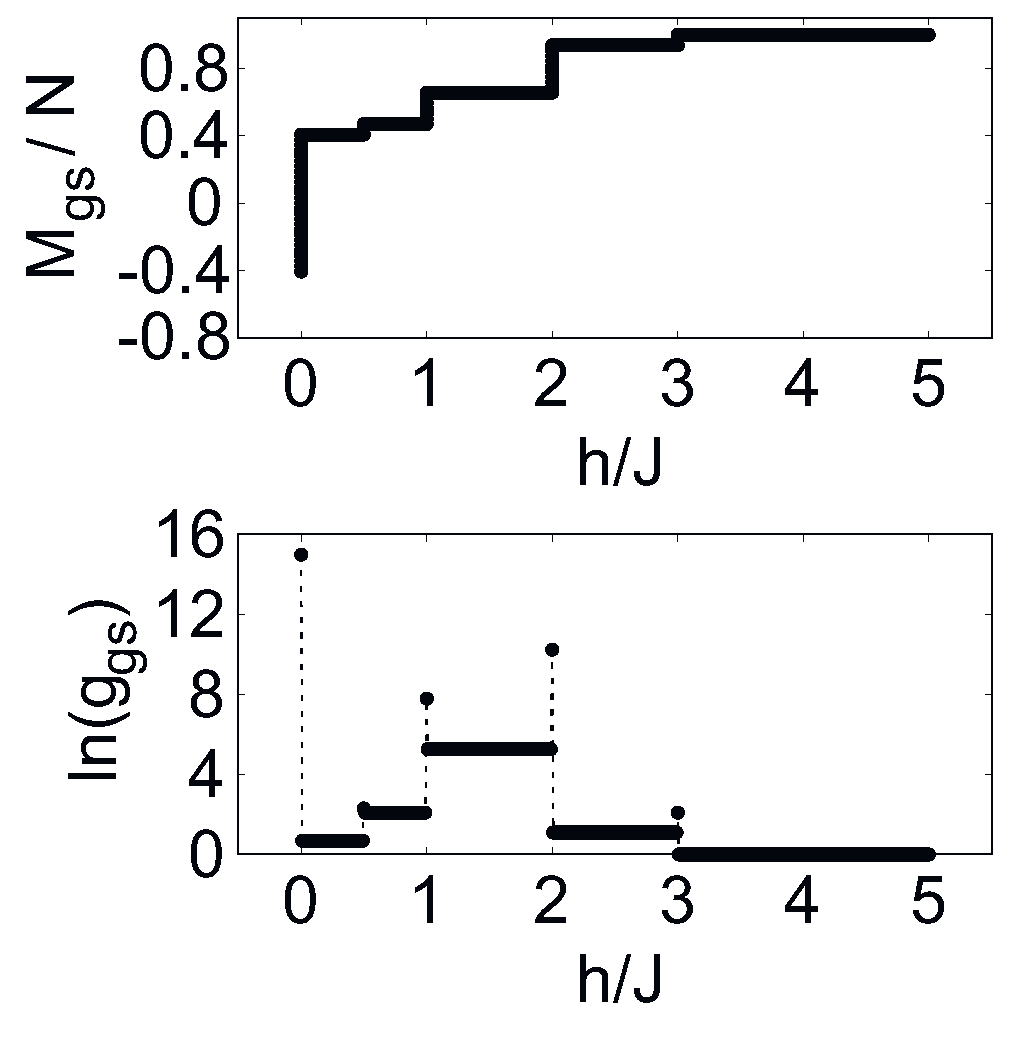
\includegraphics[width=1\linewidth]{pictures/_multiplot_SI64_J0}
	\end{minipage}
	
	\caption{Спиновый лед (a, c) и спиновое стекло (b), 64 спина, $P_+ = 0.5$}
	\label{fig:_multiplot_SI_SG_64}
	
\end{figure}


На рисунке \ref{fig:_multiplot_SI_SG_64} представлены зависимости спинового избытка и вырождения основного состояния от значения напряженности внешнего магнитного поля. 
При отсутствии фрустраций и внешнего магнитного поля основное состояние спинового льда вырождено дважды (рисунок \ref{fig:_multiplot_SI_SG_64}(a)).
В спиновом стекле с появлением фрустраций вырождение основного состояния достигает 64 (рисунок \ref{fig:_multiplot_SI_SG_64}(b)).
Максимальное заполнение системы спинового льда фрустрированными плакетами 2-го типа приводит к макроскопическому вырождению основного состояния, количество вырождений достигает 3211264 конфигураций (рисунок \ref{fig:_multiplot_SI_SG_64}(c)).



При воздействии внешнего магнитного поля больше всего ступенек на графике спинового избытка наблюдается в системе спинового стекла (рисунок \ref{fig:_multiplot_SI_SG_64}(b)). Причем их количество обуславливается не множеством фрустраций, а формой плотности распределения состояний (DOS), которая играет важную роль.
Стоит заметить, что количество ступенек неявным образом зависит от числа фрустраций.


Методом исчерпывающего перечисления для образцов спинового льда и спинового стекла, представленных на рис. \ref{fig:cell_SI_SG_64}, были построены плотности распределения состояний в зависимости от значений внешнего магнитного поля (рис. \ref{fig:HDOS_ice_1}, \ref{fig:HDOS_glass} и \ref{fig:HDOS_ice}).
Энергия системы с учетом воздействия внешнего магнитного поля вычислялась по формуле (\ref{eq:ising_energy}).




\begin{figure}[H]
	\centering
	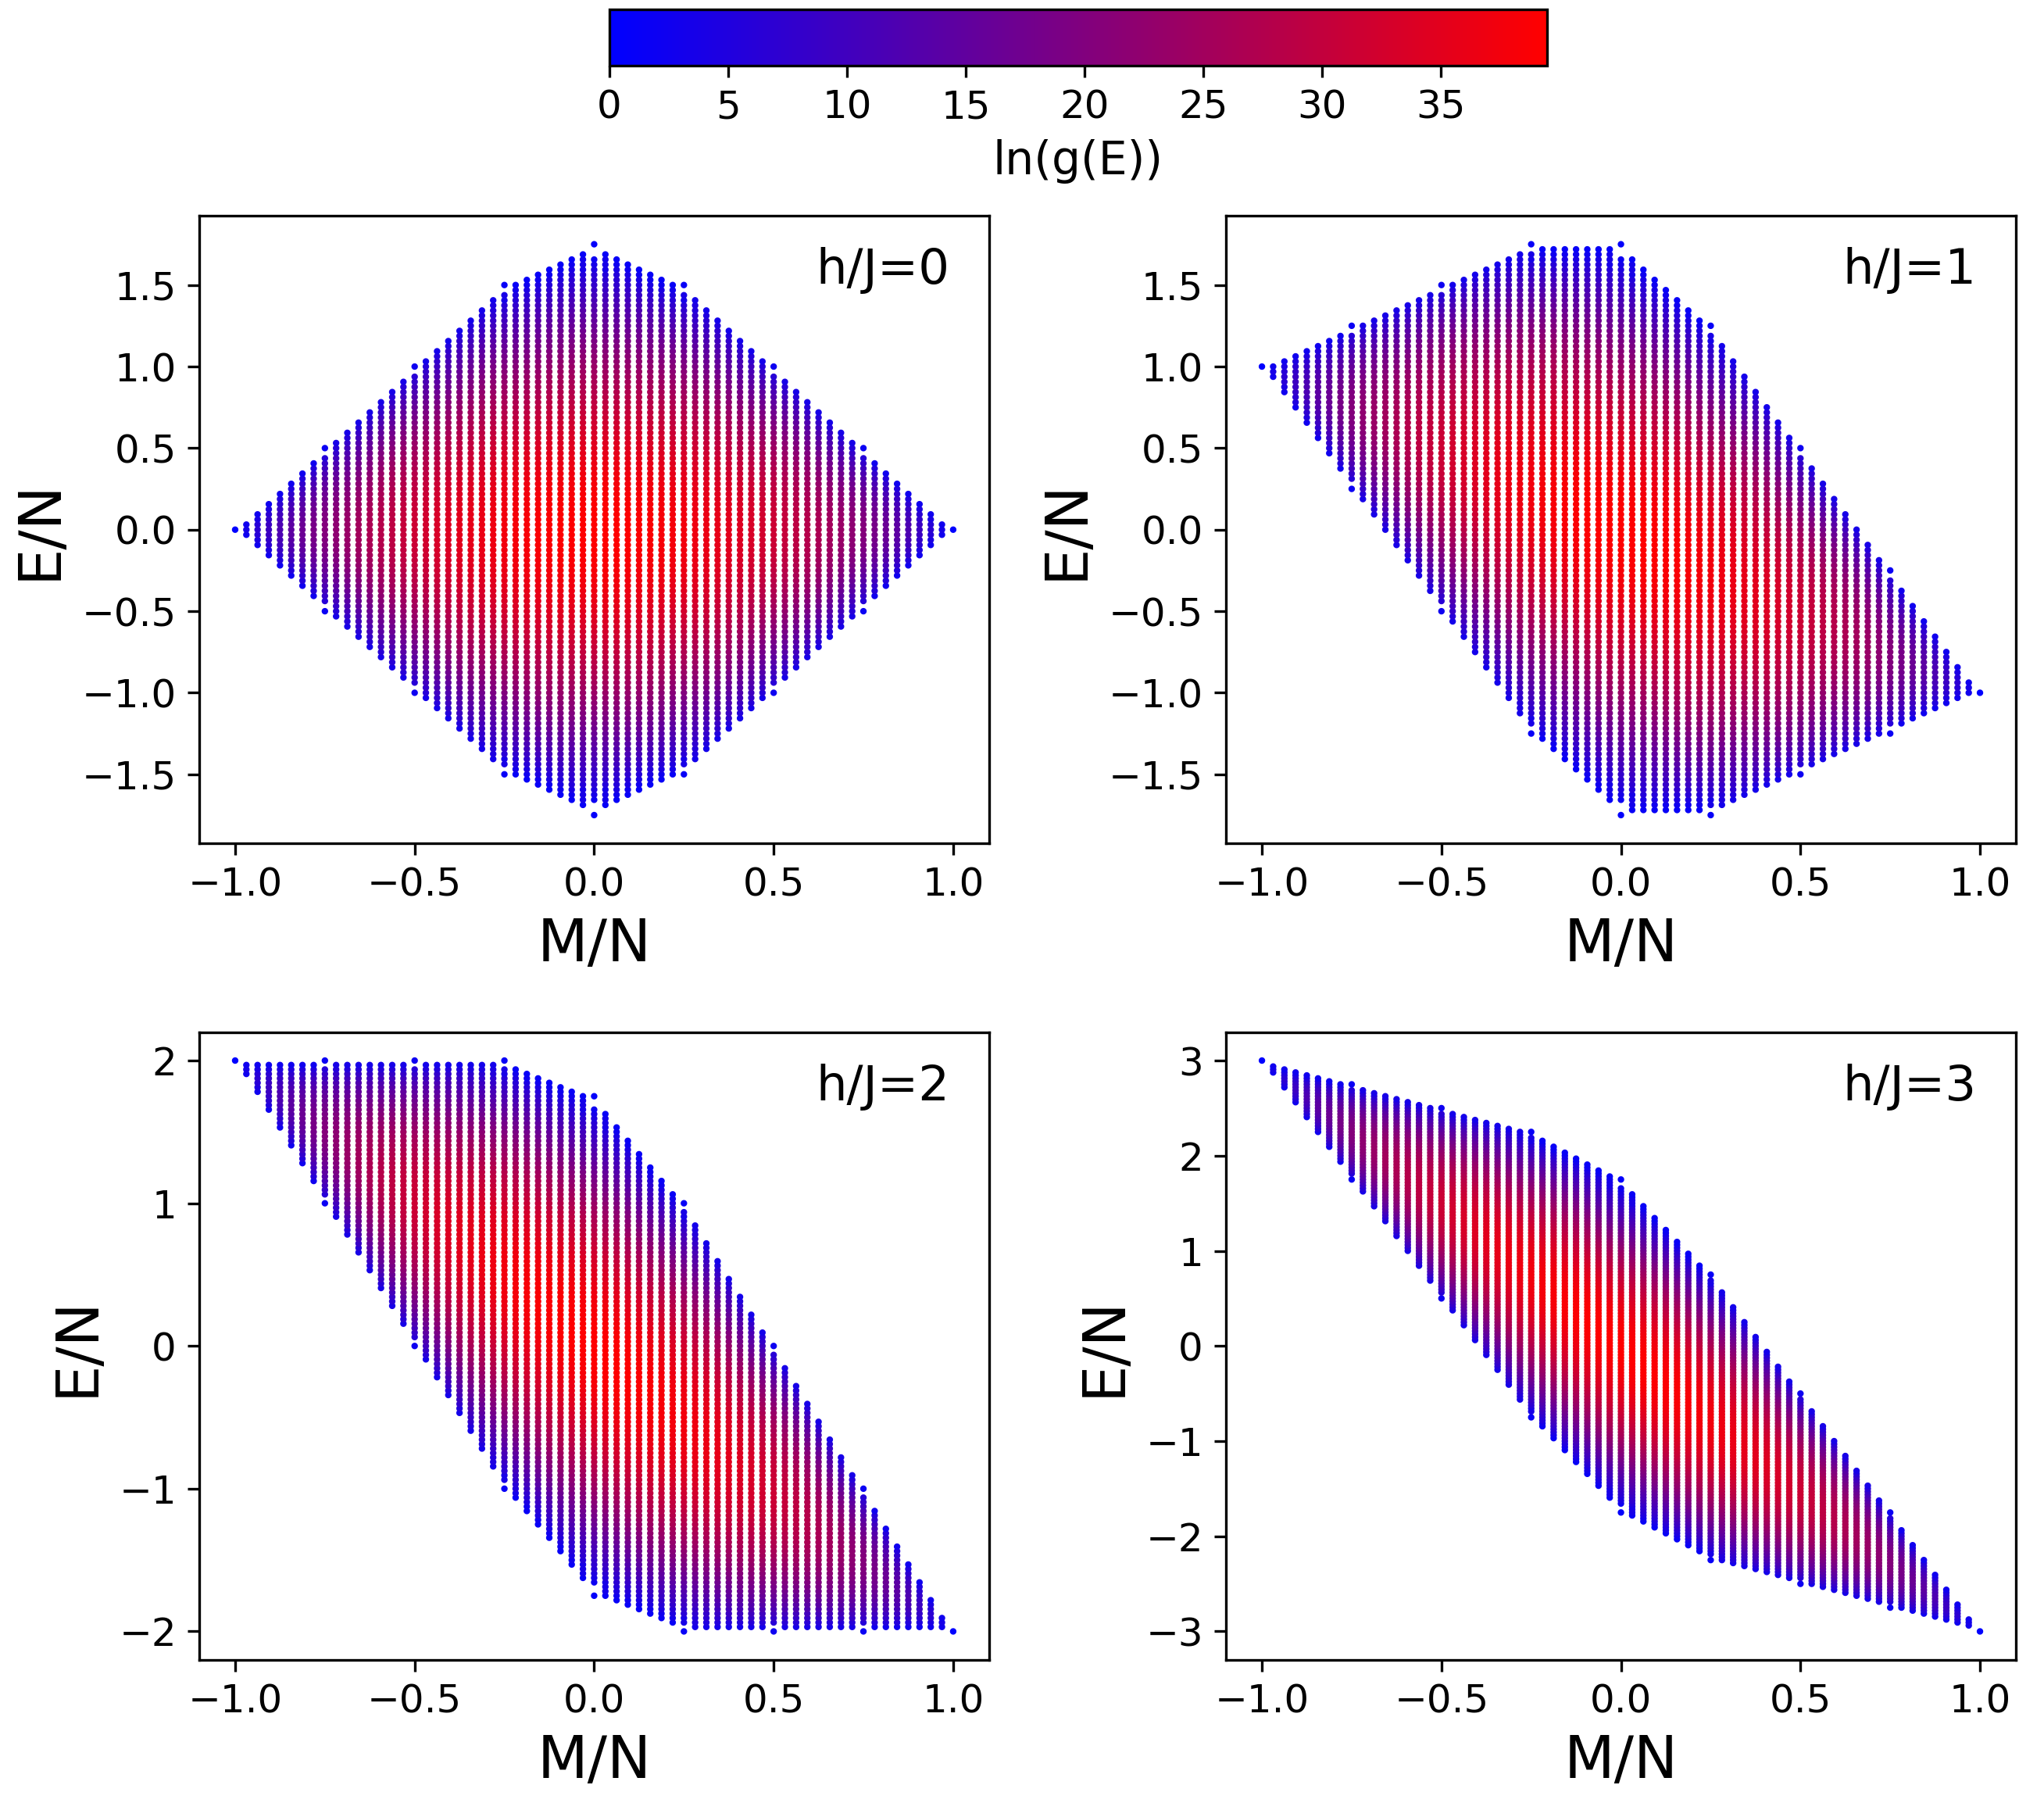
\includegraphics[width=1\linewidth]{pictures/HDOS_SI_64_J0_1.png}
	\caption{Плотность состояний во внешнем магнитном поле $0\leq h/J \leq 2$ решетки спинового льда (распределение обменных констант на рис. \ref{fig:_multiplot_SI_SG_64}(a))}
	\label{fig:HDOS_ice_1}
\end{figure}




\begin{figure}[H]
		\centering
		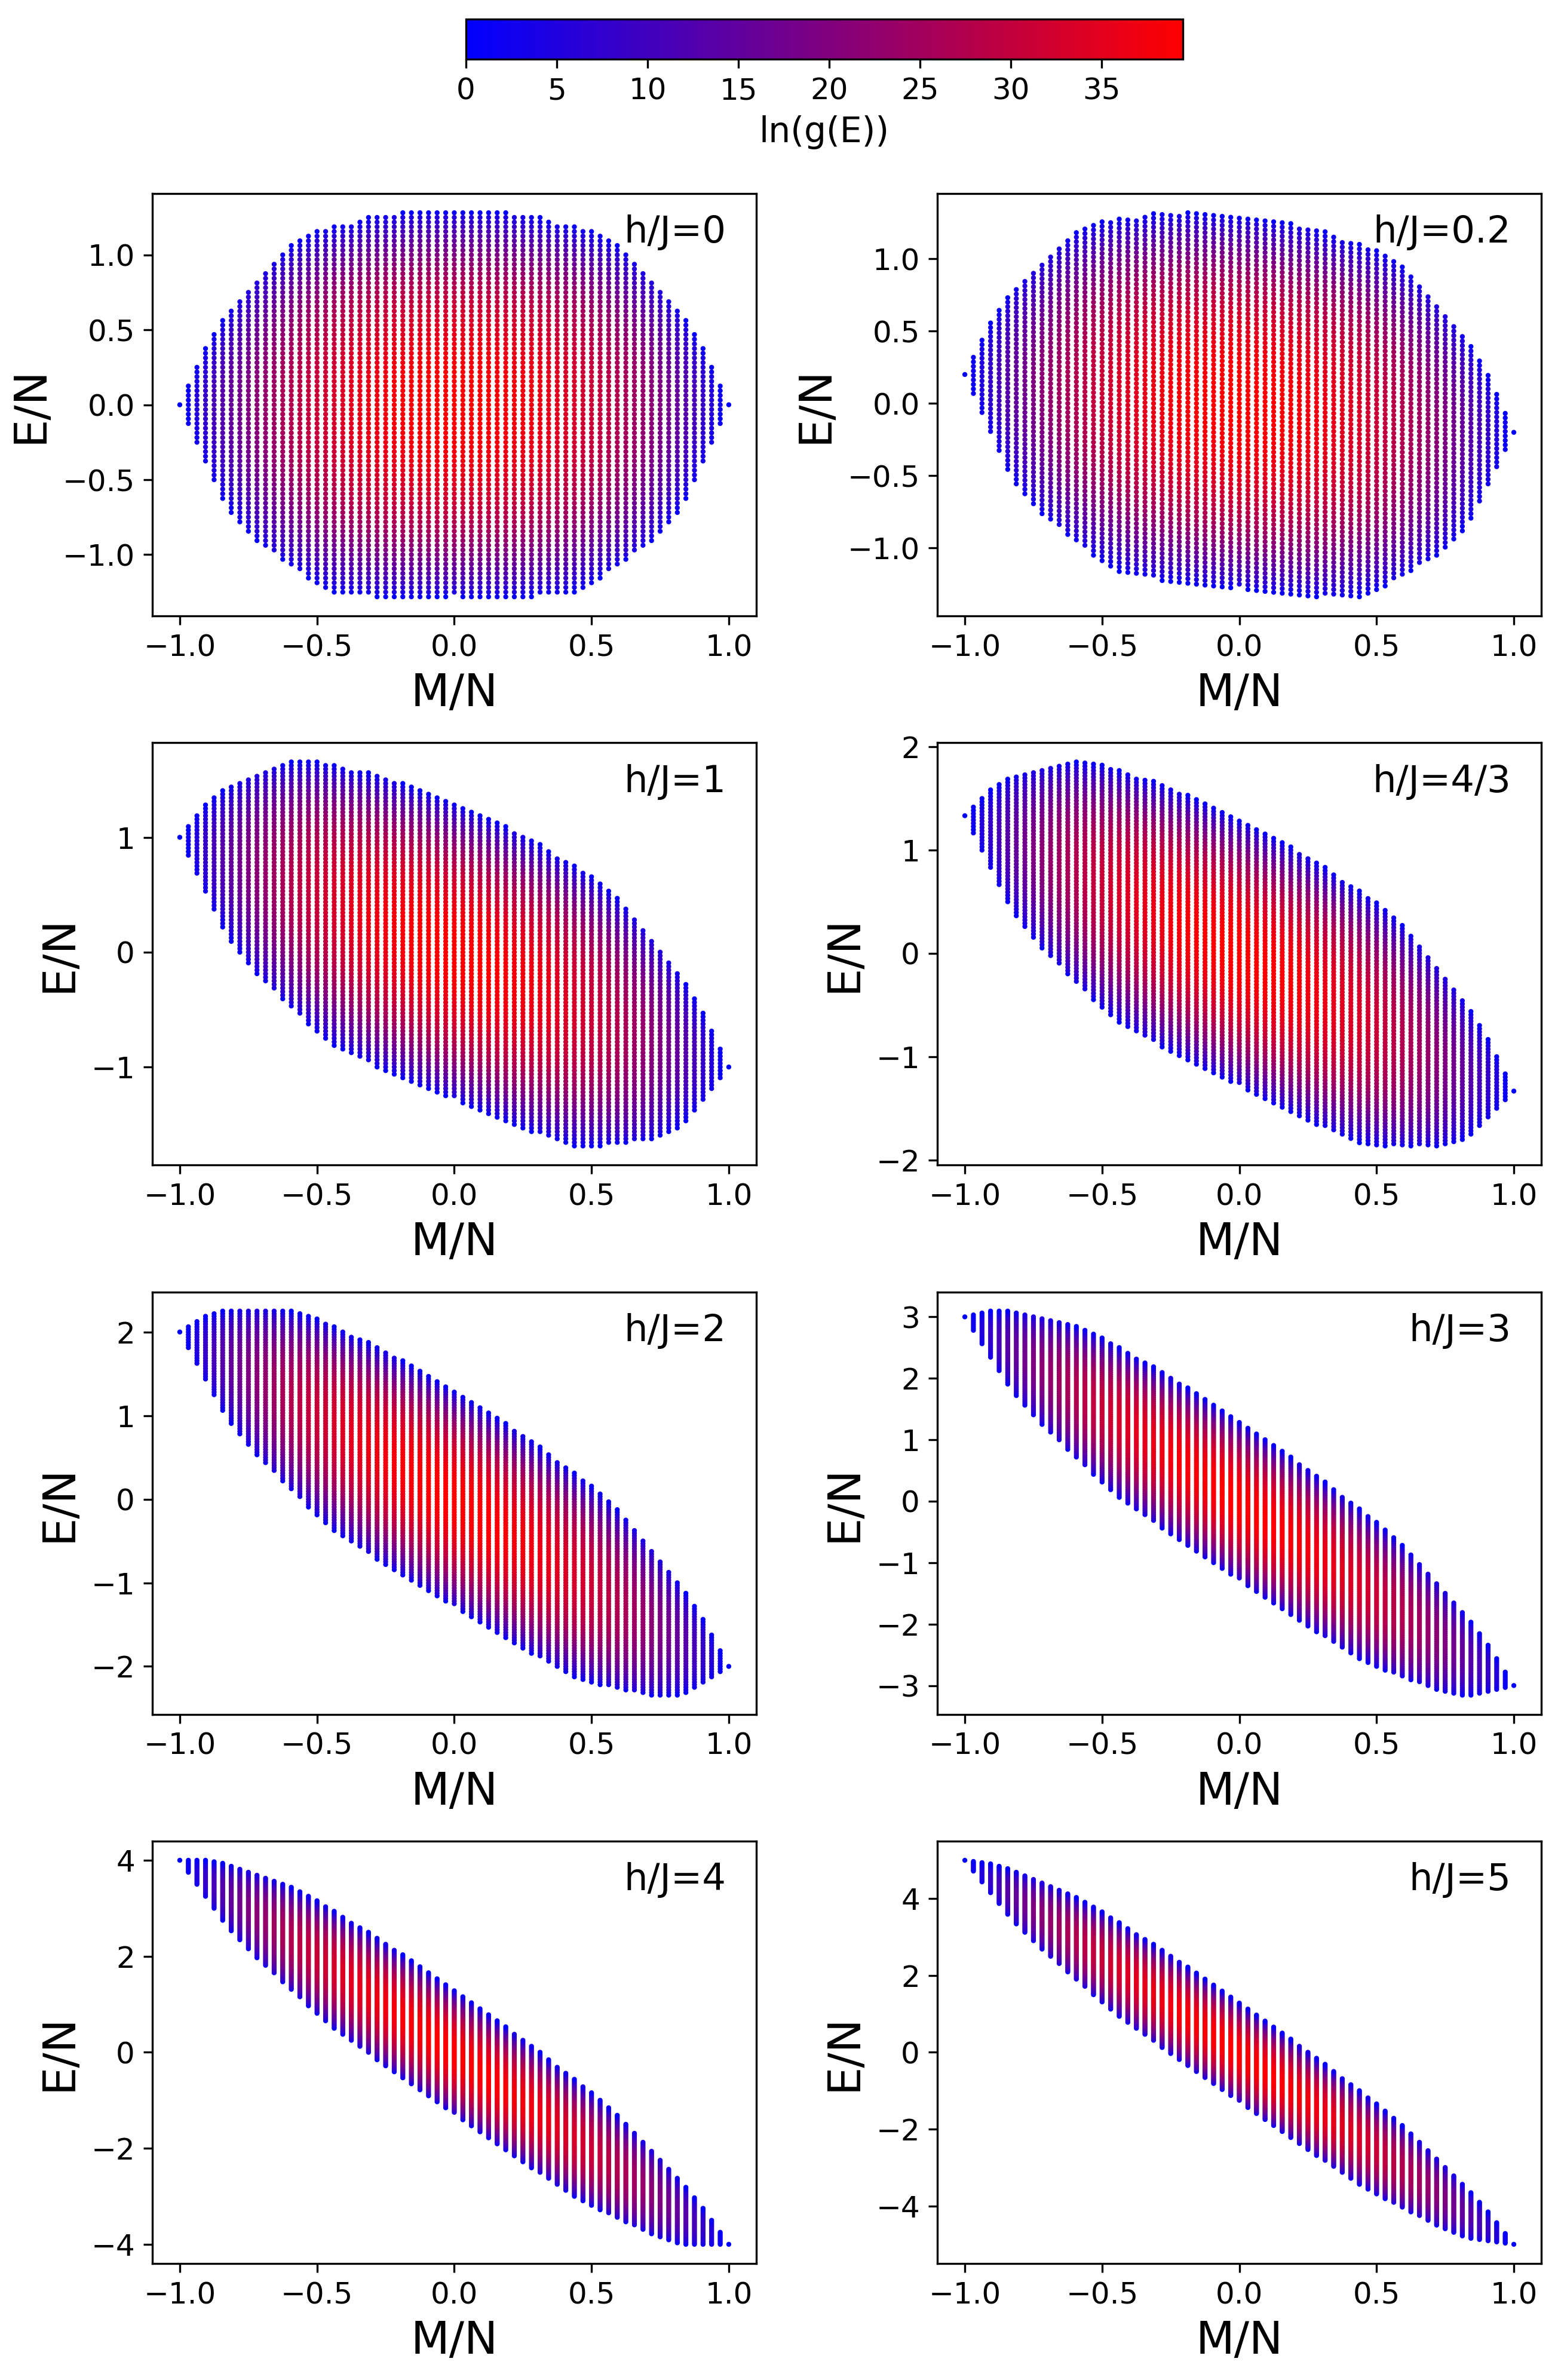
\includegraphics[width=1\linewidth]{pictures/HDOS_SG_64_J0.png}
	\caption{Плотность состояний во внешнем магнитном поле $0\leq h/J \leq 5$ решетки спинового стекла (распределение обменных констант на рис. \ref{fig:_multiplot_SI_SG_64}(b))}
	\label{fig:HDOS_glass}
\end{figure}


\begin{figure}[H]
	\centering
	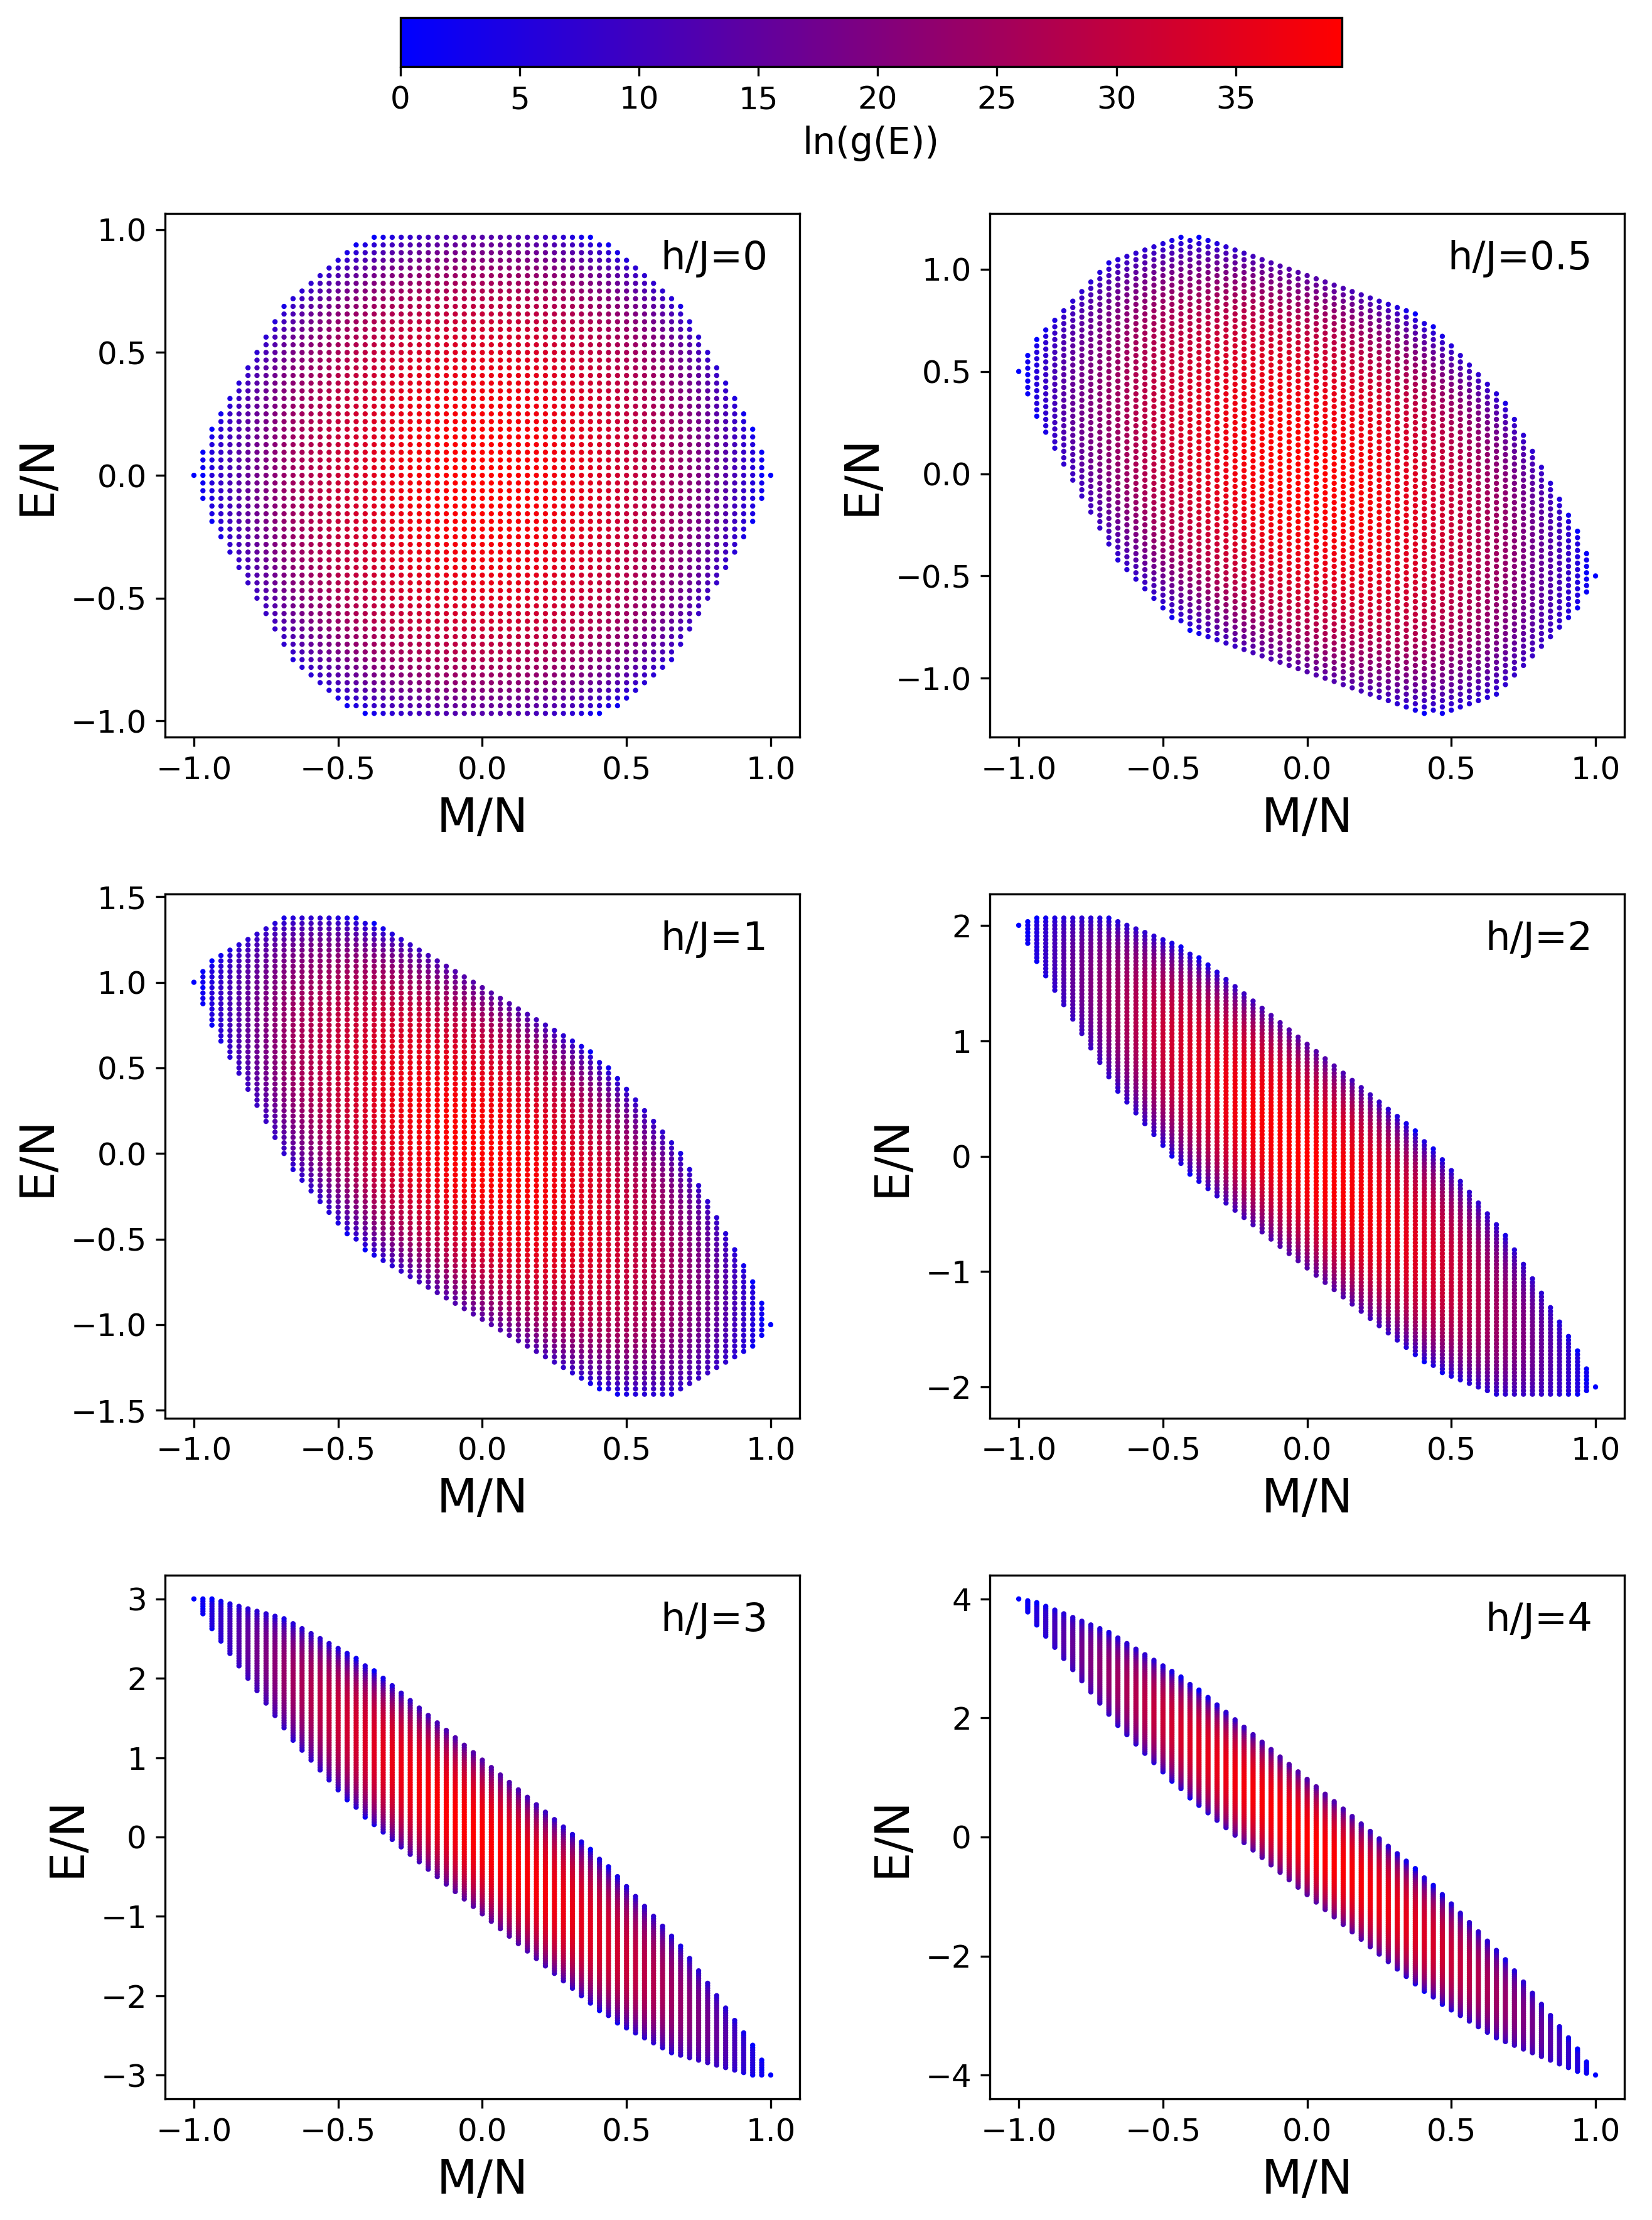
\includegraphics[width=1\linewidth]{pictures/HDOS_SI_64_J0.png}
	\caption{Плотность состояний во внешнем магнитном поле $0\leq h/J \leq 4$ решетки спинового льда (распределение обменных констант на рис. \ref{fig:_multiplot_SI_SG_64}(c))}
	\label{fig:HDOS_ice}
\end{figure}


Как мы можем видеть на рисунке \ref{fig:HDOS_ice_1} при $h/J=0$ для спинового льда (рис. \ref{fig:cell_SI_SG_64}(a)) можно видеть вырождение основного состояния. Увеличение значения внешнего магнитного поля до критического значения $h/J=1$ за счет увеличения энергии Зеемана приводит к тому, что значение энергии основного состояния со спиновым избытком $M=0$ становится равным значению энергии основного состояния со спиновым избытком $M=0.25$. Энтропии основных состояний складываются.
Увеличение значения внешнего магнитного поля до $h/J=2$ приводит к ситуации, когда основными состояниями становятся состояния со спиновыми избытками $M=\pm0.25; \pm0.5; \pm0.75; \pm1$.
Значение  $h/J=3$ есть поле насыщения, при котором остается только одна конфигурация.


Для спинового стекла (рис. \ref{fig:cell_SI_SG_64}(b)) скачки энтропии при $T=0$ в критических полях обусловлены границами плотности состояний (см. рис. \ref{fig:HDOS_glass}).


Спиновый лед (рис. \ref{fig:cell_SI_SG_64}(c)) имеет не такое большое разнообразие критических полей в отличие от спинового стекла (см. рис. \ref{fig:HDOS_ice}). Однако вырождение основных состояний больше, чем в спиновом стекле.


\section{Антиферромагнетизм, спиновое стекло и ферромагнетизм при $T = 0$}

В работе \cite{trukhin4855337thermodynamic} определена фазовая диаграмма при отличной от нуля температуре во внешнем магнитном поле. Представляет интерес вопрос разделения фаз антиферромагнетика, спинового стекла и ферромагнетика при $T=0$.

В таблице \ref{tab:lit_phase} приведены данные теоретических и численных расчётов критической точки перехода (относительная концентрация ферромагнитных связей $P_+$) из фазы антиферромагнетика в фазу спинового стекла.

\begin{table}[!h]
	\begin{tabular}{|l|c|l|}
		\hline
		Method                                   & $P_{+}$                                       & Reference                                           
		\\ \hline
		Series expansion 								& ~0.099                                  & \cite{PhysRevB.19.260}    \\ \hline
	     Matching algorithm                            & 
	     0.105 $\pm 0.01$                                        & \cite{H_Freund_1989} \\ \hline
		Matching algorithm                      & 
		$0.095<p_c<0.108$                                          & \cite{BENDISCH1994139}      \\ \hline
		Exact ground states                       & 
		$0.106 \pm 0.002$                               & \cite{N.Kawashima_1997}     \\ \hline
		Ground state enumeration                             & 0.115                                          & \cite{PhysRevE.58.1502} \\ \hline
    	Exact ground states        & 
		$0.1031\pm0.0001$                                          & \cite{WANG200331}   \\ \hline
		Exact ground states   & $0.103\pm0.001$                                       & \cite{amoruso2004domain} 
		    \\ \hline
			
	\end{tabular}
	\caption{Критическая точка для перехода AFM-SG, концентрация ферромагнитных связей}
	\label{tab:lit_phase}
\end{table}

На рисунке \ref{fig:Mgs(P+)} представлена диаграмма спиновых избытков основного состояния образцов квадратной решетки Изинга, которая получена на основе данных исчерпывающего перечисления. Плотность распределения ферромагнитных связей определяется параметром $P_+$. Связи распределены случайным образом с сохранением $P_+$ для одной серии. Каждая серия содержала \textbf{10 образцов} для численного расчёта. 

\begin{figure}[H]
	\centering
	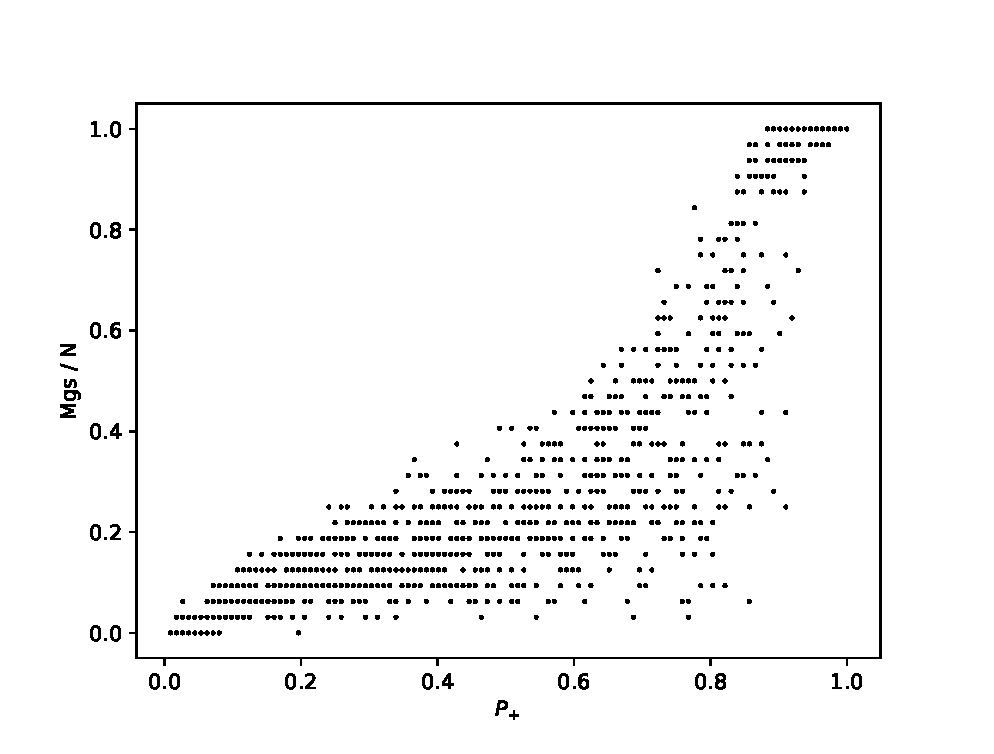
\includegraphics[width=0.8\textwidth]{images/Mgs(P+).eps}
	\caption{Значения максимального спинового избытка основного состояния в зависимости от относительного количества ферромагнитных связей $P_+$}
	\label{fig:Mgs(P+)}
\end{figure}

Очевидно, что для чистого ферромагнетика ($P_+ = 1.0$) спиновый избыток будет равен количеству спинов ($M/N = 1.0$), а для чистого антиферромагнетика -- нулю (в случае чётного количества спинов). Для каждого заданного $P_+$ отношение числа точек, в которых максимальный спиновый избыток основного состояния равен нулю, к числу точек, где $M_{gs}/N \neq 0.0$, есть вероятность антиферромагнитного состояния, рис. \ref{fig:P_AFM_FM_Mmax} (a). Аналогичным образом, отношение числа точек с $M_{gs}/N = 1.0$ ферромагнитных спиновых избытков основного состояния к числу точек, когда $M_{gs}/N \neq 1.0$, есть вероятность ферромагнитного состояния, рис. \ref{fig:P_AFM_FM_Mmax} (b).

\begin{figure}[H]
	\begin{minipage}[h]{0.45\linewidth}
		\centering $(a)$
		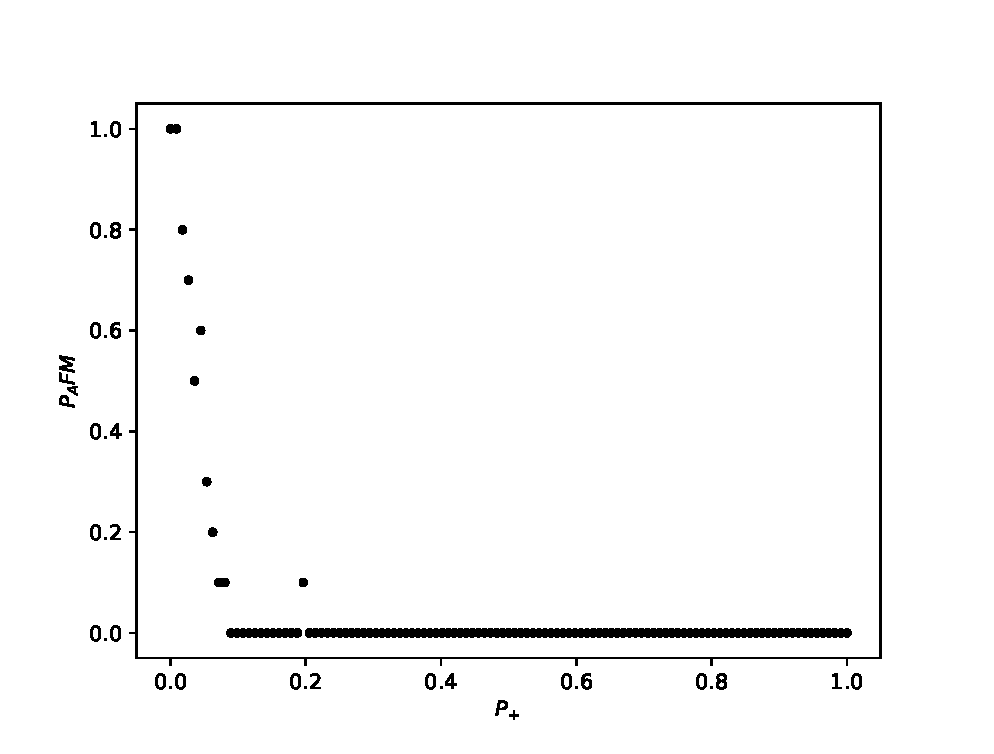
\includegraphics[width=1\linewidth]{images/P_AFM_Mmax.eps}
	\end{minipage}
	\hfill
	\begin{minipage}[h]{0.45\linewidth}
		\centering $(b)$
		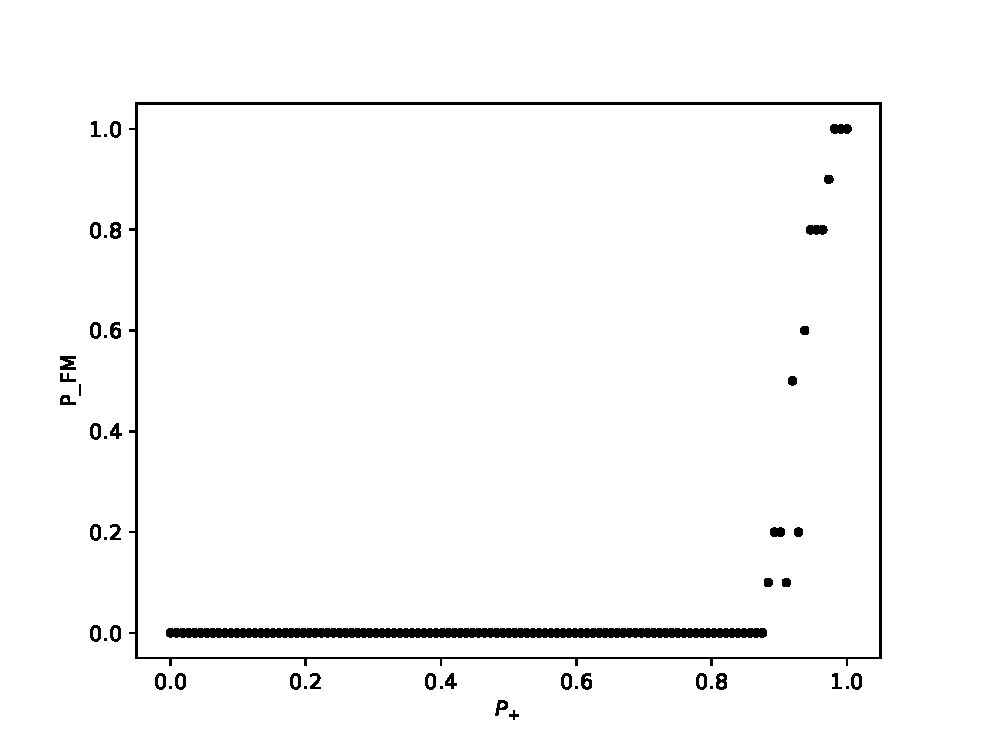
\includegraphics[width=1\linewidth]{images/P_FM_Mmax.eps}
	\end{minipage}
	\caption{Вероятность антиферромагнитного (a) и ферромагнитного (b) состояний при $T = 0$}
	\label{fig:P_AFM_FM_Mmax}
\end{figure}

Антиферромагнитная фаза при $T = 0$ реализуется при $0.0 \leq P_+ \leq 0.1$. Спиновое стекло реализуется при $0.1 \leq P_+ \leq 0.9$. Ферромагнитная фаза реализуется при $0.9 \leq P_+ \leq 1.0$. Полученные значения отделяют антиферромагнитную фазу в тех же значениях $P_+$, что и в работах, представленных в таблице \ref{tab:lit_phase}, а также позволяют отделить ферромагнитную фазу в нулевой температуре в отсутствие внешнего магнитного поля.

Полная плотность состояний позволяет достоверно рассчитать свойства образцов во внешнем магнитном поле. Под действием внешнего магнитного поля ($h/J = 1$ и $h/J = 2$) доля ферромагнитной фазы увеличивается, доля антиферромагнитной фазы уменьшается, рис. \ref{fig:Mgs(P+)_H}. Точки перехода фаз во внешнем магнитном поле ведут себя схожим образом в работе \cite{trukhin4855337thermodynamic}

\begin{figure}[H]
	\begin{minipage}[h]{0.45\linewidth}
		\centering $(a)$
		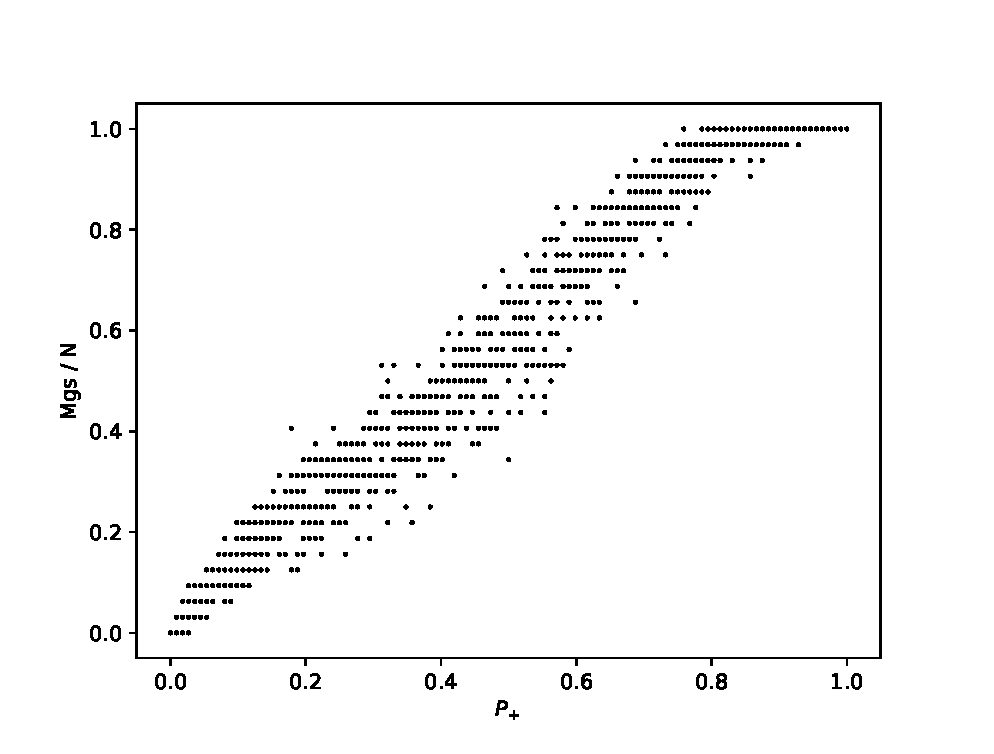
\includegraphics[width=1\linewidth]{images/Mgs(P+)_H1.eps}
	\end{minipage}
	\hfill
	\begin{minipage}[h]{0.45\linewidth}
		\centering $(b)$
		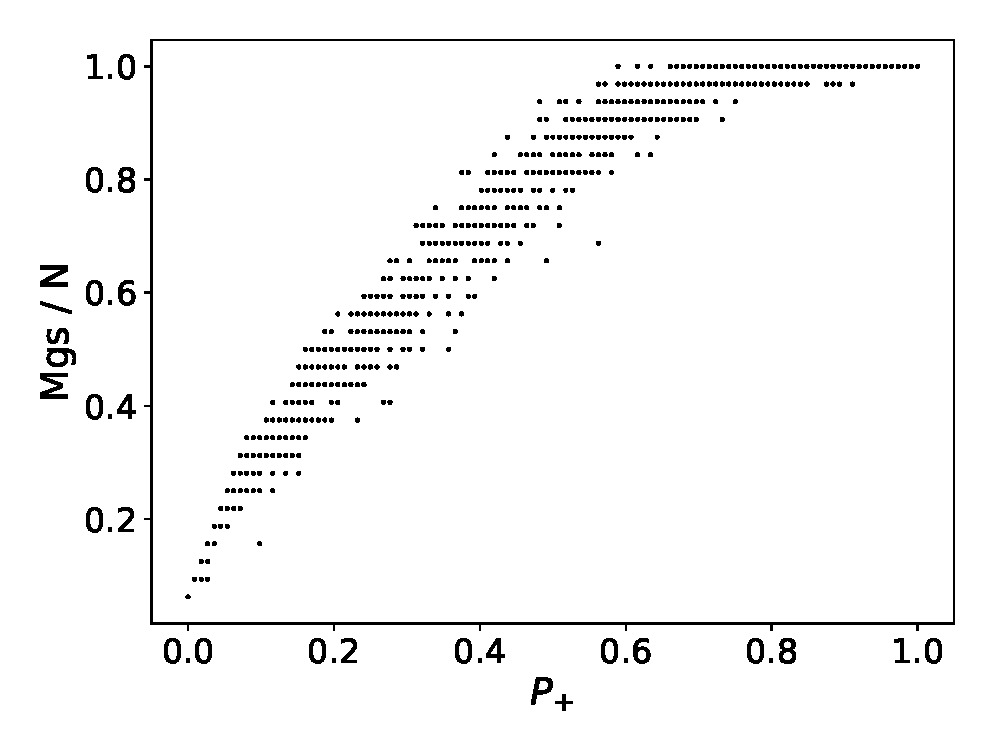
\includegraphics[width=1\linewidth]{images/Mgs(P+)_H2.eps}
	\end{minipage}
	\caption{Спиновый избыток основного состояния для всех значений плотности распределения обменных интегралов во внешнем магнитном поле $h/J = 1$ (a) и $h/J = 2$ (b)}
	\label{fig:Mgs(P+)_H}
\end{figure}

Теоретическая фазовая диаграмма $h -- P_+$ основного состояния представлена на рисунке \ref{fig:P+_afm_fm(H)}).  

\begin{figure}[H]
	\centering
	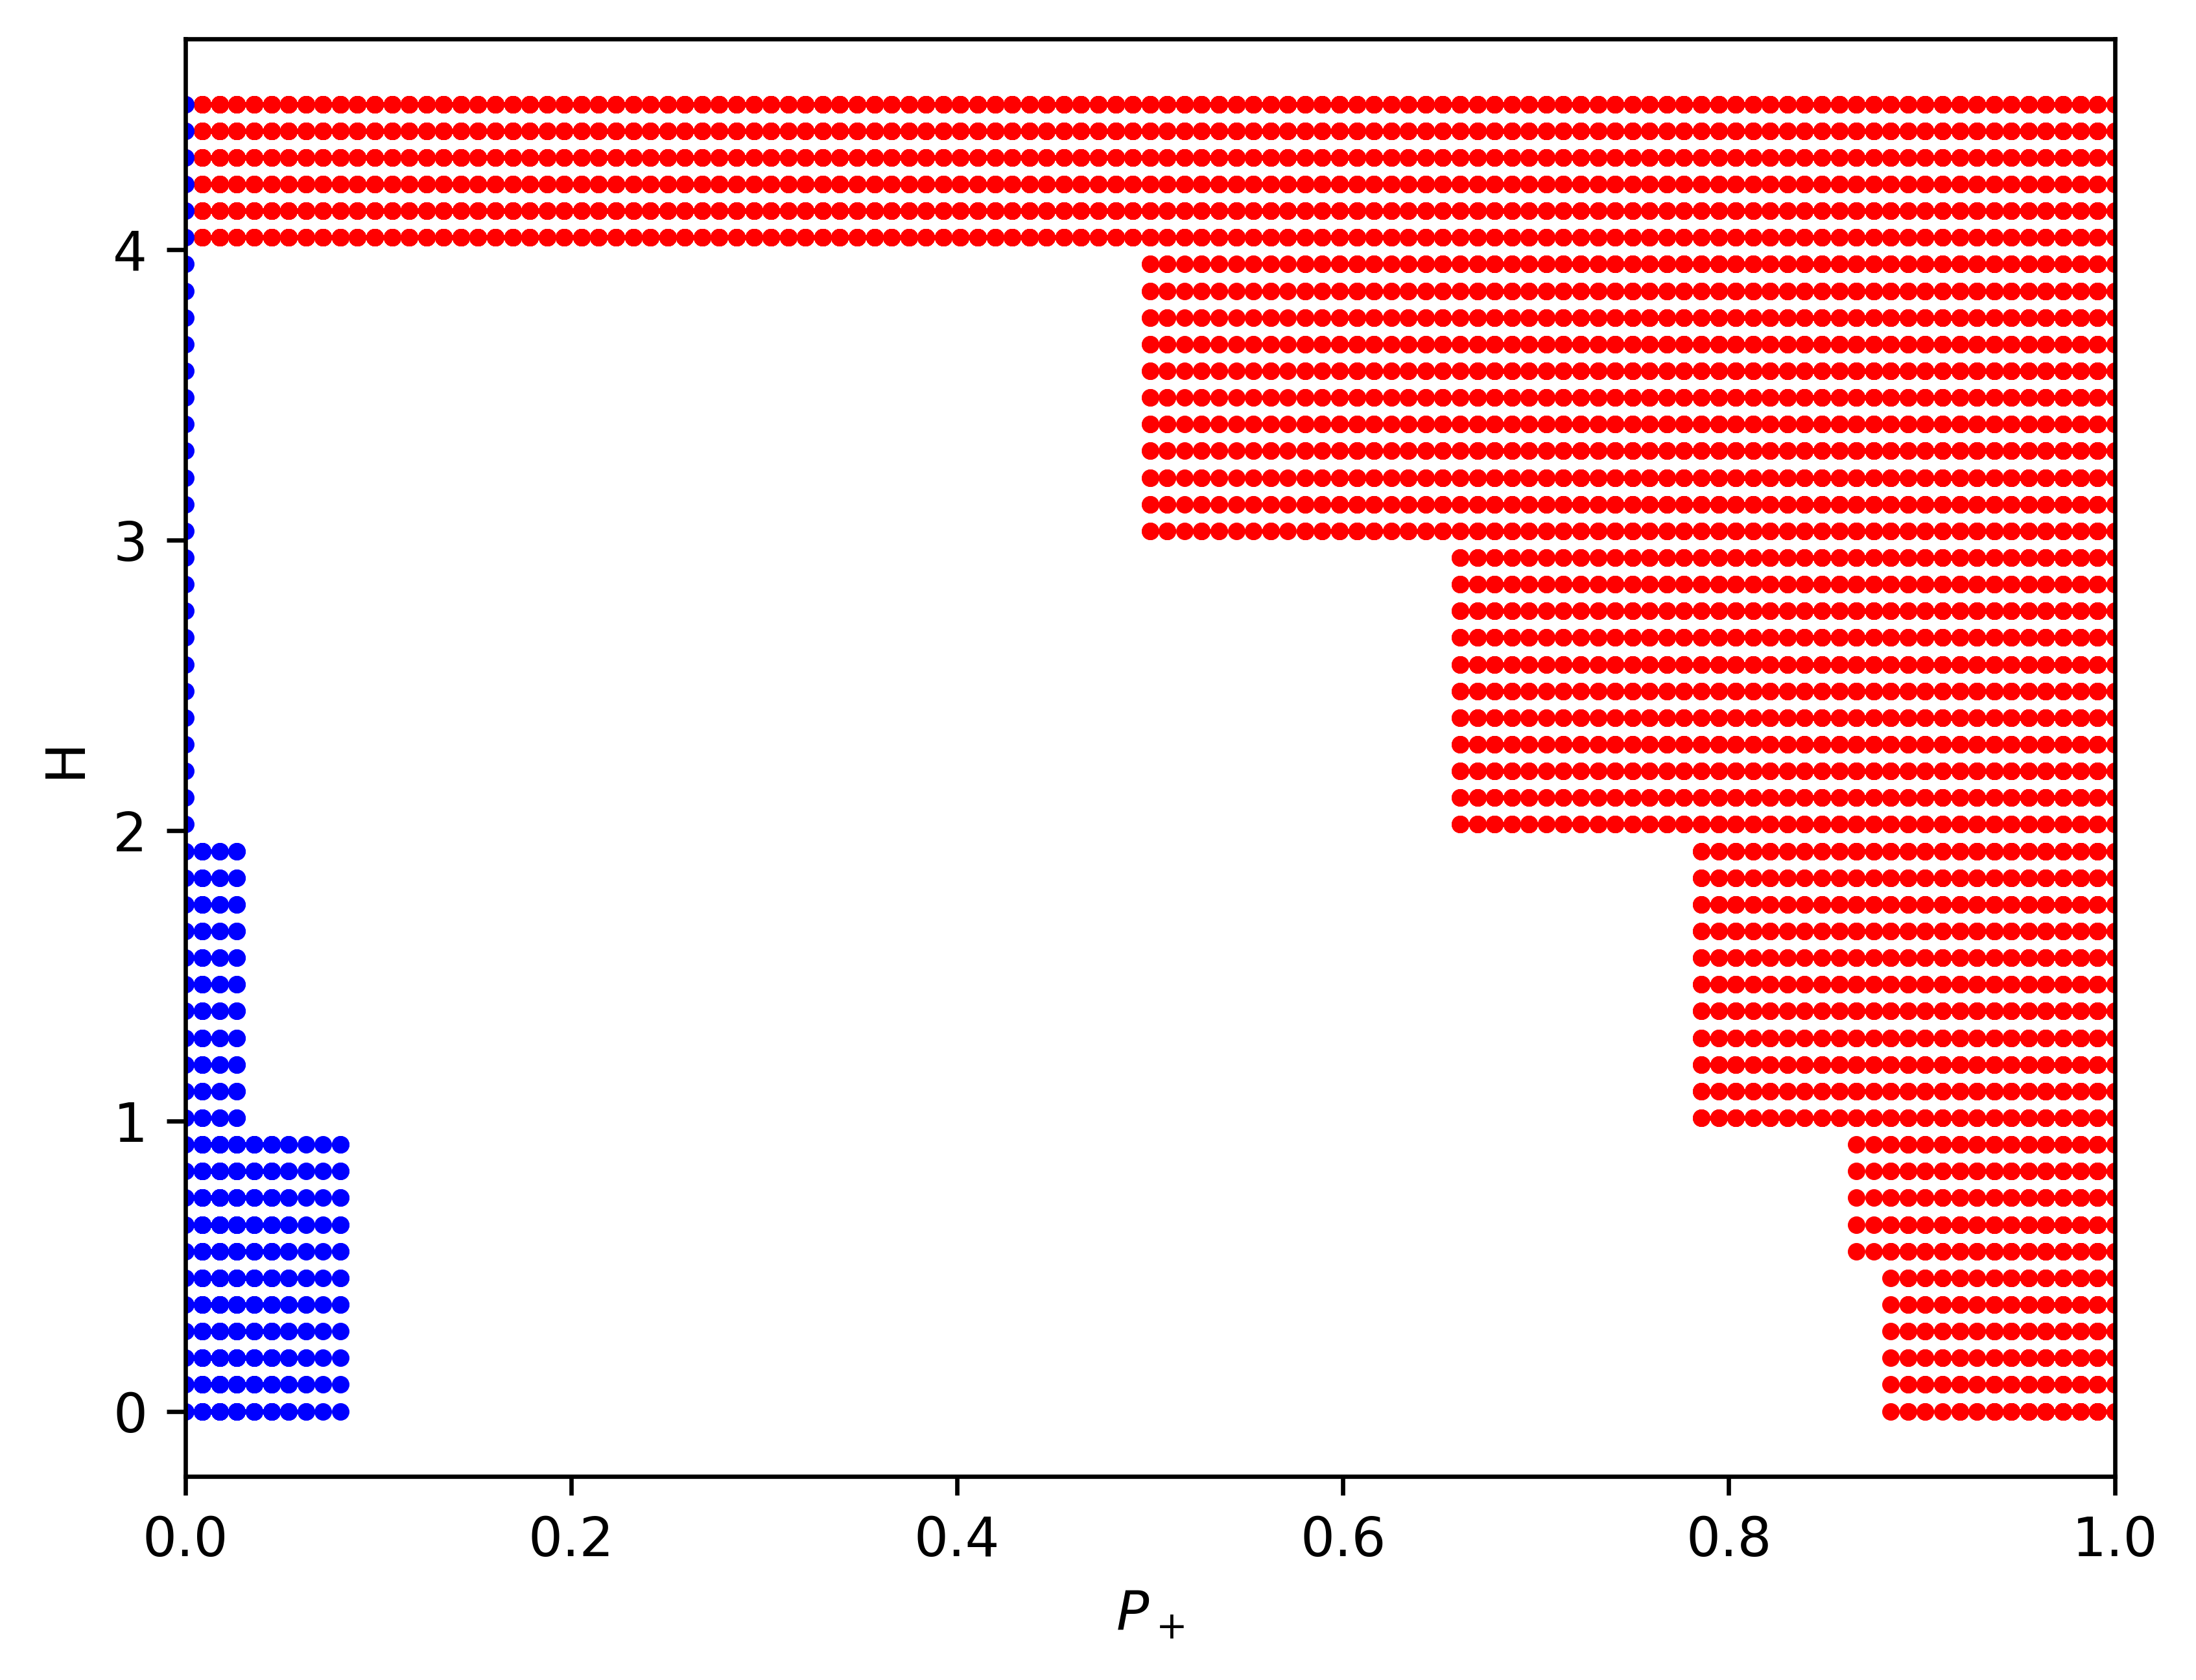
\includegraphics[width=0.8\textwidth]{images/P+_afm_fm(H)_filled.png}
	\caption{Приблизительное разделение фаз при $T = 0$ во внешнем магнитном поле. Синие точки -- фаза антиферромагнетика, красные -- ферромагнетика. Точки это отличная от нуля вероятность того, что $M/N = 0$ или $M/N = 1$, для антиферромагнетика и ферромагнетика, соответственно TODO:подписать фазы}
	\label{fig:P+_afm_fm(H)}
\end{figure}

Включение внешнего магнитного поля приводит к смещению границ существования фаз. Так для антиферромагнетика в поле $H/J > 1$ происходит спин-флоп для части образцов, в поле $H/J > 2$ -- для всех.

Из диаграммы следует что во внешнем магнитном поле $H/J > 4$ все образцы переходят в состояние ферромагнетика. 

Ступенеобразное поведения диаграммы может быть объяснено конкуренцией энергии внутренних взаимодействий ($E = -\sum J_{ij} S_i S_j$) и энергии Зеймана ($E = - h \sum S_i$). При определённых значниях поля энергия Зеймана перевешивает внутренние энергии приводит к фазовому переходу целой группы образцов с разными  $P_+$.

Необходимо отметить что открытые граничные условия могут внести существенные искажения в полученные результаты. Так один образец с $P_+ = 0.2$ (рис. \ref{fig:Mgs(P+)}, \ref{fig:P_AFM_FM_Mmax}) показывает свойства антиферромагнетика за счёт того что ферромагнитные связи $J_{ij} = 1$ располагаются вдоль границы.

\section{Заключение}

Точное решение для основного состояния модели Эдвардса-Андерсона на простой квадратной решетке 8х8 спинов получено и исследовано методом исчерпывающего перечисления. Разработанный авторский алгоритм позволяет рассчитать вырождение, энергию и спиновый избыток для каждого из $2^N$ возможных состояний, провести исследования при отсутствии температуры, выполнить поиск основного состояния при $T=0$ и отличном от нуля внешнем магнитном поле $h/J$. 

Показано, что в модели Эдвардса-Андерсона для исследуемых образцов конечного размера макроскопическое вырождение основного состояния фрустрированных спиновых систем обусловлено комбинаторикой фрустрированных плакетов, т.е. количеством вариантов размещения фрустрированных пар спинов на решетке. Мы предложили алгоритм расчета энергии, спинового избытка и конфигураций основного состояния, который основан на определении расположения фрустраций. Алгоритм расчета основных состояний имеет ограничения, которые накладываются количеством возможных вариантов размещения фрустраций. 

Установлено, что плакеты 2-го типа являются единственной причиной возникновения фрустраций в основном состоянии в отсутствии внешнего магнитного поля. В конфигурациях  минимума энергии фрустрации могут также располагаться между плакетами 2-го типа или между фрустрированным плакетом и краем решётки в зависимости от расстояний и граничных условий. Макроскопическое вырождение основного состояния подразумевает альтернативные варианты размещения фрустраций.

Зависимость спинового избытка основного состояния в модели Эдвардса-Андерсона от внешнего магнитного поля при $T\rightarrow 0$ имеет дискретный (ступенчатообразный, лестничный) характер. Такое поведение обусловлено дискретной структурой плотности состояний. Вычислены критические значения внешнего магнитного поля, при которых наблюдаются гигантские скачки остаточной энтропии. Природа скачков энтропии обусловлена тем, что при определенных критических значениях внешнего магнитного поля сумма нескольких конфигураций спинов с разной энергией взаимодействия и энергией Зеемана, т.е. с разным значением спинового избытка, будут обладать одинаковой полной энергией. Кратности вырождения состояний с одинаковой полной энергией суммируются.


Задача о максимальном количестве фрустраций в зависимости от количества спинов в системе для заданного типа решетки в модели Изинга с антиферромагнитным и ферромагнитным обменным взаимодействием может иметь интерес, поскольку наличие фрустраций приводит к появлению новых свойств. Показано, что в модели Эдвардса-Андерсона существуют системы с двукратным вырождением основного состояния, при этом в конфигурациях минимума энергии существуют фрустрации. Кроме того, может представлять интерес задача о размещении фрустраций в конфигурациях основного состояния (т.е. задача о вырождении состояний с отличным от нуля спиновым избытком), задача о подавлении фрустраций внешним магнитным полем. 


\section{Благодарности}

Исследование выполнено за счет гранта Российского научного фонда № 24-71-10069, https://rscf.ru/project/24-71-10069/.

The research was supported by the Russian Science Foundation grant No. 24-71-10069, https://rscf.ru/en/project/24-71-10069/.

\bibliography{mybibfile}


\end{document}